\documentclass[12pt,a4paper]{article}
\usepackage[utf8]{inputenc}
\usepackage[T1]{fontenc}
\usepackage{graphicx}
\usepackage{booktabs}
\usepackage{geometry}
\usepackage{hyperref}
\usepackage{amsmath}
% natbib removed - using standard cite
\usepackage{caption}
\usepackage{subcaption}
\usepackage{xcolor}
\usepackage{float}

\geometry{margin=2.5cm}

\title{Seismic Risk Assessment of Dam Infrastructure in Myanmar \\
Following the 2025 Mandalay Earthquake (M$_w$ 7.7)}

\author{
  Aung Khant Zaw\textsuperscript{1} \\[0.5em]
  \textsuperscript{1}Independent Researcher, Myanmar \\[0.5em]
  \texttt{aungkhantzawd@gmail.com}
}

\date{\today}

\begin{document}

\maketitle

\begin{abstract}
Myanmar's 254 documented dams face significant seismic hazard from the active Sagaing Fault and other tectonic structures.
The March 28, 2025 Mandalay earthquake (M$_w$ 7.7) at 10~km depth produced one of the longest strike-slip ruptures ever recorded (500~km), reaching a peak ground acceleration of 1.07$g$ in Naypyidaw and damaging 586 dams according to government assessments.
We present a comprehensive seismic risk assessment integrating 9,242 earthquake events (1970--2026) from the Myanmar Earthquake API with georeferenced dam data from the Open Development Mekong database.
A corrected Gutenberg-Richter analysis above the true magnitude of completeness ($M_c$ = 4.0) yields a b-value of 0.71 $\pm$ 0.02, consistent with moderately elevated seismic hazard.
Using UTM-projected DBSCAN spatial clustering, we identify seven distinct seismic zones along the Sagaing Fault system, with the Central Myanmar cluster accounting for 8,775 events and a maximum recorded magnitude of M$_w$ 7.7.
Peak Ground Acceleration at each dam site is estimated using the Abrahamson \& Silva (2008) NGA-West1 ground motion prediction equation for crustal strike-slip earthquakes, with Joyner-Boore distance ($R_{jb}$) measured to the nearest fault trace rather than to the epicenter, properly accounting for the 500~km extended rupture.
PGA values range from 0.022$g$ to 0.201$g$ (mean: 0.062$g$) using site-specific $V_{S30}$ (600--1,100~m/s, mean: 968~m/s) estimated from the Copernicus DEM via the Wald \& Allen (2007) slope-based proxy.
A composite risk scoring framework incorporating PGA, fault proximity, mainshock proximity, and structural exposure classifies 25 dams (9.8\%) at \textit{Critical} risk and 119 (46.9\%) at \textit{High} risk.
Monte Carlo sensitivity analysis with 100 random weight combinations confirms that the Critical and High categories are robust to weight perturbation, with the combined Critical+High fraction ranging from 30--70\% across all weight combinations.
Probabilistic seismic hazard analysis (PSHA) yields a mean 475-year PGA of 0.31$g$ across all dam sites, with 32 dams (12.6\%) exceeding 0.5$g$ at the 10\% in 50-year exceedance level.
The Modified Omori law fit to the aftershock sequence gives a decay parameter $p = 0.83$.
Our results indicate that over 56\% of Myanmar's documented dams are located in zones of significant seismic hazard, warranting urgent structural evaluation and monitoring.
All data, code, and interactive visualizations are published as open-source tools.
\end{abstract}

\noindent\textbf{Keywords:} seismic hazard, dam safety, Myanmar, Sagaing Fault, PGA, Abrahamson \& Silva, NGA, risk assessment, 2025 Mandalay earthquake

\section{Introduction}

Myanmar occupies one of the most seismically active regions in Southeast Asia, situated at the boundary between the Indian, Eurasian, Burma, and Sunda tectonic plates.
The northward-moving Indian plate converges with the Eurasian plate at approximately 35~mm/year, producing right-lateral strike-slip motion along the $\sim$1,400~km Sagaing Fault that bisects the country from north to south \cite{vigny2003present,wang2014active}.
GPS measurements indicate the Sagaing Fault accommodates approximately 18~mm/year of this motion \cite{socquet2006myanmar}.
The fault passes through or near major population centers including Mandalay, Naypyidaw, and Yangon, and has been described as an ``earthquake superhighway'' due to its potential for supershear ruptures \cite{robinson2010earthquake}.

Historical earthquakes along the Sagaing Fault include the 1930 Bago (M$_w$ 7.5) and Pyu (M$_w$ 7.3) events, the 1946 Sagaing doublet (M$_w$ 7.3 and 7.7), the 1956 Sagaing earthquake (M$_w$ 7.1), the 1991 event (M$_w$ 7.0), and the 2012 Shwebo earthquake (M$_w$ 6.8) \cite{wang2014active}.

On March 28, 2025, the M$_w$ 7.7 Mandalay earthquake struck at 06:20:52 UTC (12:50:52 MMT) with its epicenter near Sagaing (22.001$^\circ$N, 95.925$^\circ$E) at a shallow depth of 10~km.
The earthquake produced a 500~km surface rupture along the Meiktila, Naypyidaw, Pyu, and southern Sagaing segments of the fault, making it one of the longest strike-slip ruptures ever precisely recorded \cite{usgs2025mandalay}.
The rupture propagated at supershear velocity, with a duration of approximately 85 seconds and maximum slip of 5--7~m.
A USGS seismic station in Naypyidaw recorded a peak ground acceleration of 0.623$g$ and a GFZ station recorded 1.066$g$ \cite{usgs2025mandalay}.
The event caused catastrophic damage across central Myanmar: 5,456 fatalities, 11,404 injuries, and economic losses estimated at US\$11 billion (14\% of GDP) according to World Bank assessments.
The Myanmar government reported that 586 dams were damaged or destroyed.

Myanmar's water infrastructure includes at least 254 documented dams serving irrigation (46\%), hydropower (37\%), multi-purpose (8\%), and water supply (2\%) functions.
Many of these structures were designed and built before modern seismic codes were established, and their vulnerability to strong ground motion is poorly characterized.
The 2025 event exposed critical gaps in dam safety assessment: several dams reported structural damage, and emergency evacuations were issued downstream of structures in the affected zone.

This study aims to:
(1) characterize the seismic hazard environment in Myanmar through spatial clustering and frequency-magnitude analysis with proper catalog completeness correction;
(2) estimate ground motion intensities at each dam site using a modern ground motion prediction equation calibrated for crustal strike-slip earthquakes;
(3) develop a composite risk scoring framework that integrates seismic, geometric, and structural factors, with sensitivity analysis;
(4) identify the most vulnerable dams requiring urgent safety evaluation.

\section{Study Area and Tectonic Setting}

Myanmar lies within a complex tectonic zone bounded by the actively deforming India-Eurasia collision zone.
The dominant structural feature is the Sagaing Fault, a major right-lateral transform fault running approximately N--S through central Myanmar, accommodating roughly 18~mm/year of dextral slip \cite{socquet2006myanmar,wang2014active}.
The fault connects the Andaman Sea spreading center to the Himalayan collision zone, running for over 1,400~km.
The southern section (16.5--23.5$^\circ$N) is divided into five segments: Bago, Pyu, Naypyidaw, Meiktila, and Sagaing \cite{wang2014active}.
The 2025 earthquake ruptured the Pyu, Naypyidaw, Meiktila, and southern Sagaing segments, breaking a seismic gap that had been identified by \cite{hurukawa2011two} as capable of producing a M$_w$ 7.9 earthquake.

Additional seismic sources include:
\begin{itemize}
    \item The Kabaw Fault and Sunda megathrust along the Indo-Myanmar Ranges, where the Indian plate subducts beneath the Burma plate
    \item The Shan Plateau fault system (including the Kyaukkyan and Nam Ma faults) in eastern Myanmar
    \item Intraslab seismicity from the subducted Indian plate beneath central Myanmar (e.g., the 1975 Bagan earthquake at 120~km depth)
\end{itemize}

Our dataset contains 9,242 earthquake events recorded between July 1970 and April 2026, primarily sourced from the USGS and international seismic networks through the Myanmar Earthquake API.
The spatial distribution (Figure~\ref{fig:study_area}) shows pronounced clustering along the central Sagaing Fault corridor, with secondary concentrations in the eastern Shan Plateau and northern Kachin State.

\begin{figure}[H]
    \centering
    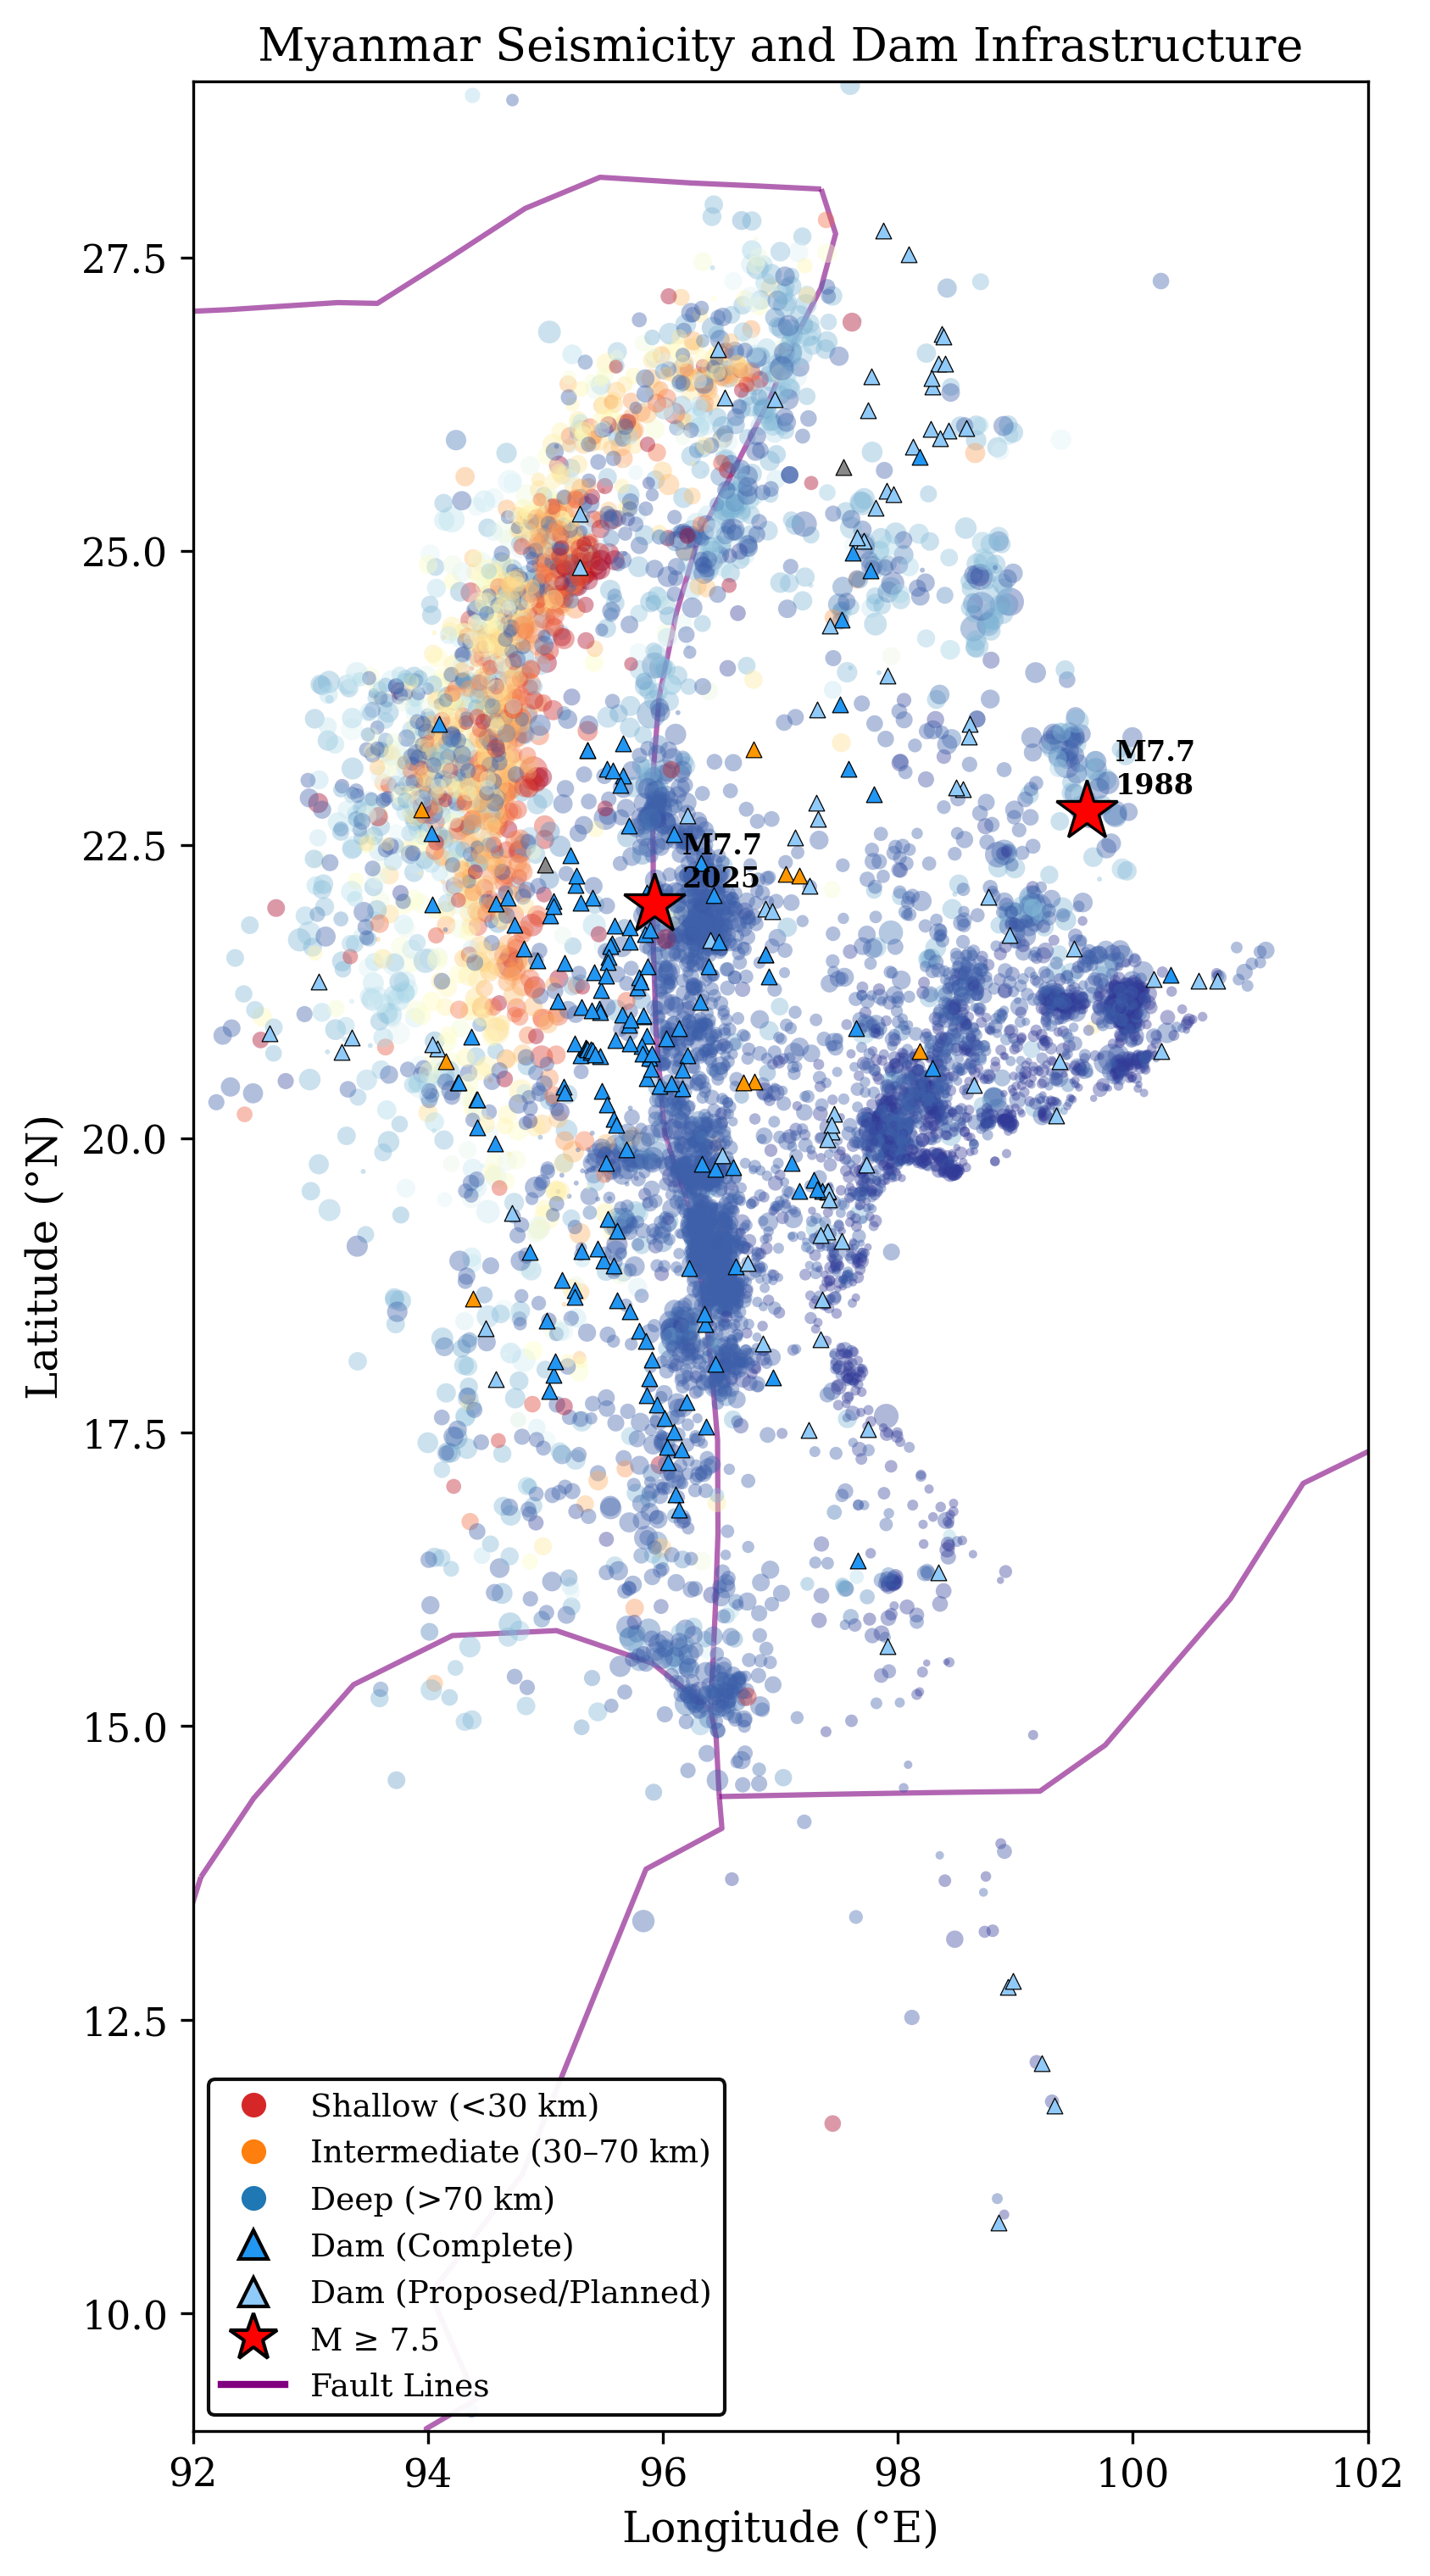
\includegraphics[width=0.9\textwidth]{figures/fig1_study_area.png}
    \caption{Study area map showing earthquake distribution (colored by depth), dam locations (triangles), major fault lines (purple), and M$\geq$7.5 events (stars, labeled with year). Note the dense clustering along the central Sagaing Fault corridor.}
    \label{fig:study_area}
\end{figure}

\section{Data and Methods}

\subsection{Earthquake Catalog}

Earthquake data was obtained from the Myanmar Earthquake API (\url{https://mmeq.akze.net}), which aggregates data from USGS, GFZ, the Thai Meteorological Department, and other regional networks.
The catalog contains 9,242 events with the following properties:
\begin{itemize}
    \item Magnitude range: M 0.0--7.7 (mean: 3.19)
    \item Depth range: 0--700~km (median: 10~km)
    \item 74.5\% shallow focus ($<$30~km), 11.8\% intermediate (30--70~km), 13.7\% deep ($>$70~km)
    \item Three events of M$\geq$7.0, 34 events of M$\geq$6.0, 284 events of M$\geq$5.0
\end{itemize}

The catalog was validated by removing events with missing coordinates, out-of-range values, or duplicate entries based on time and location proximity.

\subsection{Dam Database}

Dam data was sourced from the Open Development Mekong database \cite{odmekong2018}, which integrates datasets from the International Finance Corporation (IFC) and CGIAR's Research Program on Water, Land, and Ecosystems (WLE).
The database contains 254 dam points with metadata including project name, status, function, installed capacity, dam height, river, and administrative location.
Of these, 160 (63\%) are completed, 51 (20\%) are proposed, 14 (6\%) are planned, and 9 (4\%) are under construction (Figure~\ref{fig:dam_types}).

\begin{figure}[H]
    \centering
    
\includegraphics[width=\textwidth]{figures/fig8_dam_types.png}
    \caption{Distribution of Myanmar dams by (a) project status and (b) primary function.}
    \label{fig:dam_types}
\end{figure}

\subsection{Seismicity Analysis}

\subsubsection{Frequency-Magnitude Distribution with Catalog Completeness Correction}

We apply the Gutenberg-Richter relationship \cite{gutenberg1944frequency}:
\begin{equation}
    \log_{10} N = a - bM
    \label{eq:gr}
\end{equation}
where $N$ is the cumulative number of events of magnitude $\geq M$, $a$ is a measure of seismicity rate, and $b$ describes the relative proportion of large to small events.

A critical issue with regional catalogs spanning long time periods is that the magnitude of completeness ($M_c$) varies over time as seismic networks are upgraded.
The raw maximum curvature method \citep{wiemer2000minimum} yields $M_c$ = 2.2, but this reflects the post-2020 deployment of denser networks.
A stability analysis (Figure~\ref{fig:fmd}b) shows that the b-value only stabilizes near the global average of $b \approx 1.0$ at $M_c \approx 4.5$, indicating that the true completeness threshold for the full catalog period is $M_c \geq 4.0$.
We therefore compute b-values only for events above $M_c$ = 4.0, yielding a robust estimate for the full catalog.
Additionally, we compute multi-period b-values for the 1970--1999 and 2020--2026 sub-periods to assess catalog homogeneity.

\subsubsection{Spatial Clustering with Projected Coordinates}

We apply DBSCAN (Density-Based Spatial Clustering of Applications with Noise) \cite{ester1996density} to identify spatially coherent seismic zones.
To ensure physically correct distance calculations, earthquake coordinates are projected to UTM Zone 47N before clustering, and the $\epsilon$ parameter is set in meters ($\epsilon = 0.3^\circ \times 111$~km $= 33.3$~km).
The parameter \texttt{min\_samples} is set to 10.
Each identified cluster is labeled with its geographic region, event count, maximum magnitude, and mean depth.

\subsubsection{Aftershock Modeling}

The temporal decay of aftershocks is modeled using the Modified Omori Law \cite{utsu1961statistical}:
\begin{equation}
    n(t) = \frac{K}{(t + c)^p}
    \label{eq:omori}
\end{equation}
where $n(t)$ is the rate of aftershocks at time $t$ after the mainshock, $K$ controls aftershock productivity, $c$ is a small time offset, and $p$ describes the decay rate.
Parameters are fitted to M$\geq$3.0 aftershocks within the first 30 days following the 2025 mainshock.
We note that over 500 aftershocks were recorded by July 2025, with the strongest being M$_w$ 6.7 occurring 12 minutes after the mainshock \cite{usgs2025mandalay}; our catalog captures only a subset of these due to reporting latency.

\subsection{Ground Motion Estimation}

Peak Ground Acceleration (PGA) at each dam site is estimated using the Abrahamson \& Silva (2008) NGA-West1 ground motion prediction equation (GMPE), which was developed specifically for shallow crustal earthquakes in active tectonic regions \citep{abrahamson2008}:
\begin{equation}
    \ln(\text{PGA}) = f_{mag}(M) + (a_2 + a_3 M) \ln\sqrt{R_{jb}^2 + c_4^2} + f_{site}(V_{S30})
    \label{eq:pga}
\end{equation}
where $M$ is moment magnitude, $R_{jb}$ is the Joyner-Boore distance (shortest distance to the surface projection of the fault rupture), $c_4 = 5.6$~km is a depth scaling term, and $V_{S30}$ is the average shear-wave velocity in the top 30~m.
Coefficients for the strike-slip mechanism ($a_1 = -0.526$, $a_2 = -1.60$, $a_3 = 0.143$, $a_{10} = -0.135$, $a_{13} = -0.015$, $c_1 = 6.2$) are taken from Table~3 of \citet{abrahamson2008}.

\subsubsection{Site-Specific Vs30 Estimation}

Rather than assuming uniform rock conditions ($V_{S30}$ = 760~m/s) at all sites, we estimate site-specific $V_{S30}$ using the Wald \& Allen (2007) topographic slope proxy.
Elevation data is extracted from the Copernicus DEM at 30~m resolution, resampled to $\sim$1~km spatial resolution, and the topographic gradient is computed within a 10~km window centered on each dam.
The median slope is then mapped to $V_{S30}$ using the Wald \& Allen (2007) active tectonic classification.
The resulting $V_{S30}$ values range from 600 to 1,100~m/s (mean: 968~m/s, median: 900~m/s), with 48\% of dams classified as NEHRP B ($V_{S30}$ $>$ 760~m/s) and 52\% as NEHRP BC (Figure~\ref{fig:vs30}).
The dominance of high $V_{S30}$ values reflects the mountainous terrain surrounding most Myanmar dam sites.

\begin{figure}[H]
    \centering
    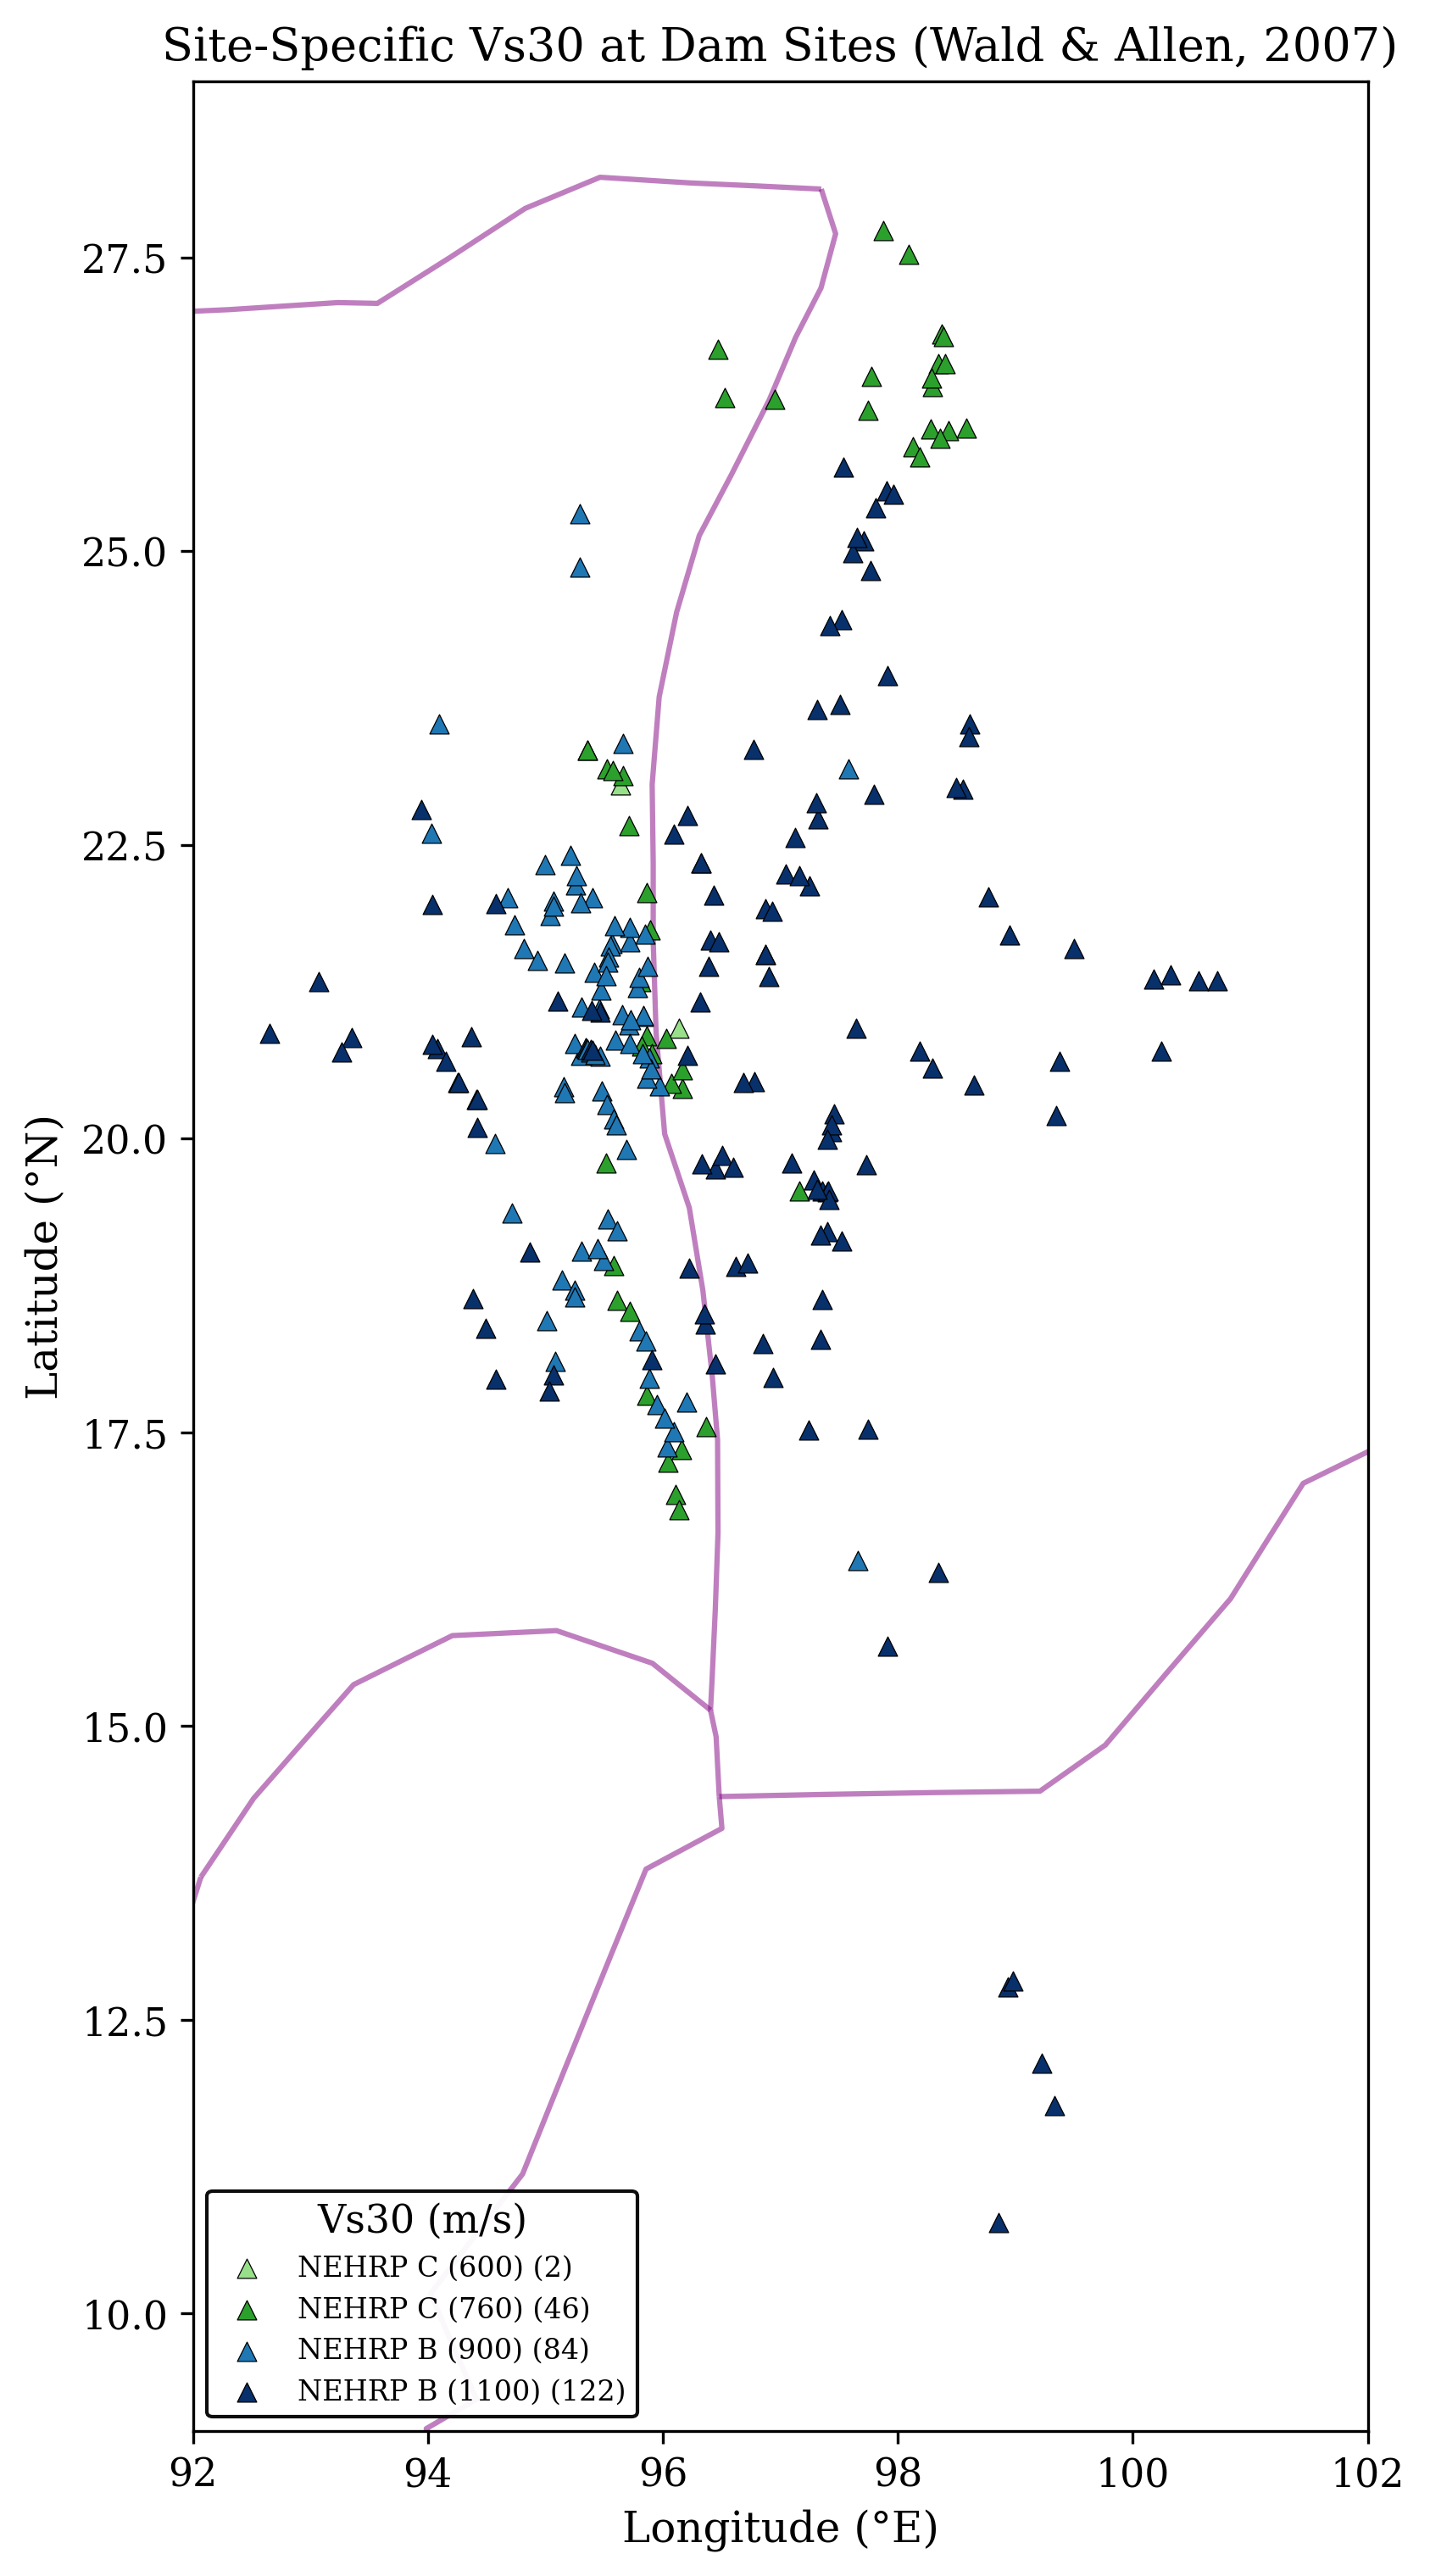
\includegraphics[width=0.9\textwidth]{figures/fig9_vs30_map.png}
    \caption{Site-specific $V_{S30}$ at dam locations estimated from Copernicus DEM using the Wald \& Allen (2007) slope-based proxy. Purple lines indicate fault traces.}
    \label{fig:vs30}
\end{figure}

This GMPE was selected over the previously used Fukushima \& Tanaka (1990) model for three reasons:
(1) it was developed for crustal strike-slip earthquakes in active tectonic regions, matching the Sagaing Fault tectonic environment;
(2) it uses $R_{jb}$ distance metric which properly accounts for extended ruptures;
(3) it is calibrated against a global dataset of strong-motion recordings including large-magnitude events.

\subsubsection{Distance Metric for Extended Ruptures}

A key consideration for the 2025 M$_w$ 7.7 event is its 500~km rupture length.
For extended ruptures, the epicentral distance is not a meaningful measure of proximity to strong shaking.
Instead, we use the Joyner-Boore distance ($R_{jb}$), defined as the shortest distance from the site to the surface projection of the fault rupture.
For each dam, $R_{jb}$ is approximated as the distance to the nearest fault trace segment from the global plate boundary dataset (Figure~\ref{fig:study_area}).
This approach correctly assigns low $R_{jb}$ values (and hence high PGA) to dams near the fault trace even if they are hundreds of km from the epicenter.

For comparison, the model median predicts PGA of 0.14--0.18$g$ at $R_{jb}$ = 5--10~km from the fault trace for M$_w$ 7.7.
The actual recordings in Naypyidaw (0.62--1.07$g$) are consistent with these median predictions when the within-event variability ($\sigma \approx 0.6$ in natural log units, or approximately a factor of 1.8) is considered, placing the recordings at approximately the 84th--95th percentile of the predicted distribution.

\subsection{Composite Risk Scoring}

A composite risk score (0--10) is computed for each dam as a weighted sum:
\begin{equation}
    R_{composite} = 0.35 \times S_{seismic} + 0.30 \times S_{fault} + 0.20 \times S_{proximity} + 0.15 \times S_{exposure}
    \label{eq:risk}
\end{equation}

\begin{itemize}
    \item \textbf{Seismic score} ($S_{seismic}$): Based on PGA from the M$_w$ 7.7 mainshock using ASK08, scaled so that 0.05$g$ $\rightarrow$ 10
    \item \textbf{Fault proximity} ($S_{fault}$): Inverse distance to nearest fault segment, scaled so that 10~km $\rightarrow$ 10
    \item \textbf{Mainshock proximity} ($S_{proximity}$): Inverse distance to M$_w$ 7.7 epicenter, scaled so that 50~km $\rightarrow$ 10
    \item \textbf{Structural exposure} ($S_{exposure}$): Function of dam height, installed capacity, and reservoir storage
\end{itemize}

Dams are classified as \textbf{Critical} ($R \geq 7$), \textbf{High} ($5 \leq R < 7$), \textbf{Moderate} ($3 \leq R < 5$), or \textbf{Low} ($R < 3$).

\subsubsection{Sensitivity Analysis}

To assess the robustness of the risk classification to weight selection, we perform a Monte Carlo sensitivity analysis with 100 iterations.
In each iteration, the four weights are drawn from a Dirichlet distribution (ensuring they sum to 1.0), and the resulting risk grade distribution is recorded.
The variability in grade counts across all iterations provides a measure of classification uncertainty (Figure~\ref{fig:risk_dist}c).

\section{Results}

\subsection{Seismicity Characteristics}

\subsubsection{Frequency-Magnitude Distribution}

The b-value stability analysis (Figure~\ref{fig:fmd}b) reveals a strong dependence on $M_c$: the apparent b-value increases from 0.31 at $M_c$ = 2.0 to 1.07 at $M_c$ = 4.5, then stabilizes near 0.9--1.0 for $M_c \geq$ 4.5.
This pattern is diagnostic of catalog incompleteness at low magnitudes: the early decades of the catalog (1970--2000) have a much higher detection threshold ($M_c \approx$ 4.5) than the post-2020 period ($M_c \approx$ 2.5).

Using the corrected completeness threshold of $M_c$ = 4.0, the full catalog yields $b = 0.71 \pm 0.02$ and $a = 6.23$ with 2,473 events above $M_c$ (Figure~\ref{fig:fmd}a).
This b-value is below the global average of $b \approx 1.0$ but is physically reasonable for a region dominated by a major plate-boundary fault with frequent moderate-to-large earthquakes.
Multi-period analysis confirms that the 1970--1999 sub-period gives $b = 1.02$ (Mc = 4.7, N = 421), while the 2020--2026 sub-period gives $b = 0.52$ (Mc = 2.5, N = 4,494), reflecting the inclusion of the 2025 M$_w$ 7.7 mainshock sequence in the latter period.

\begin{figure}[H]
    \centering
    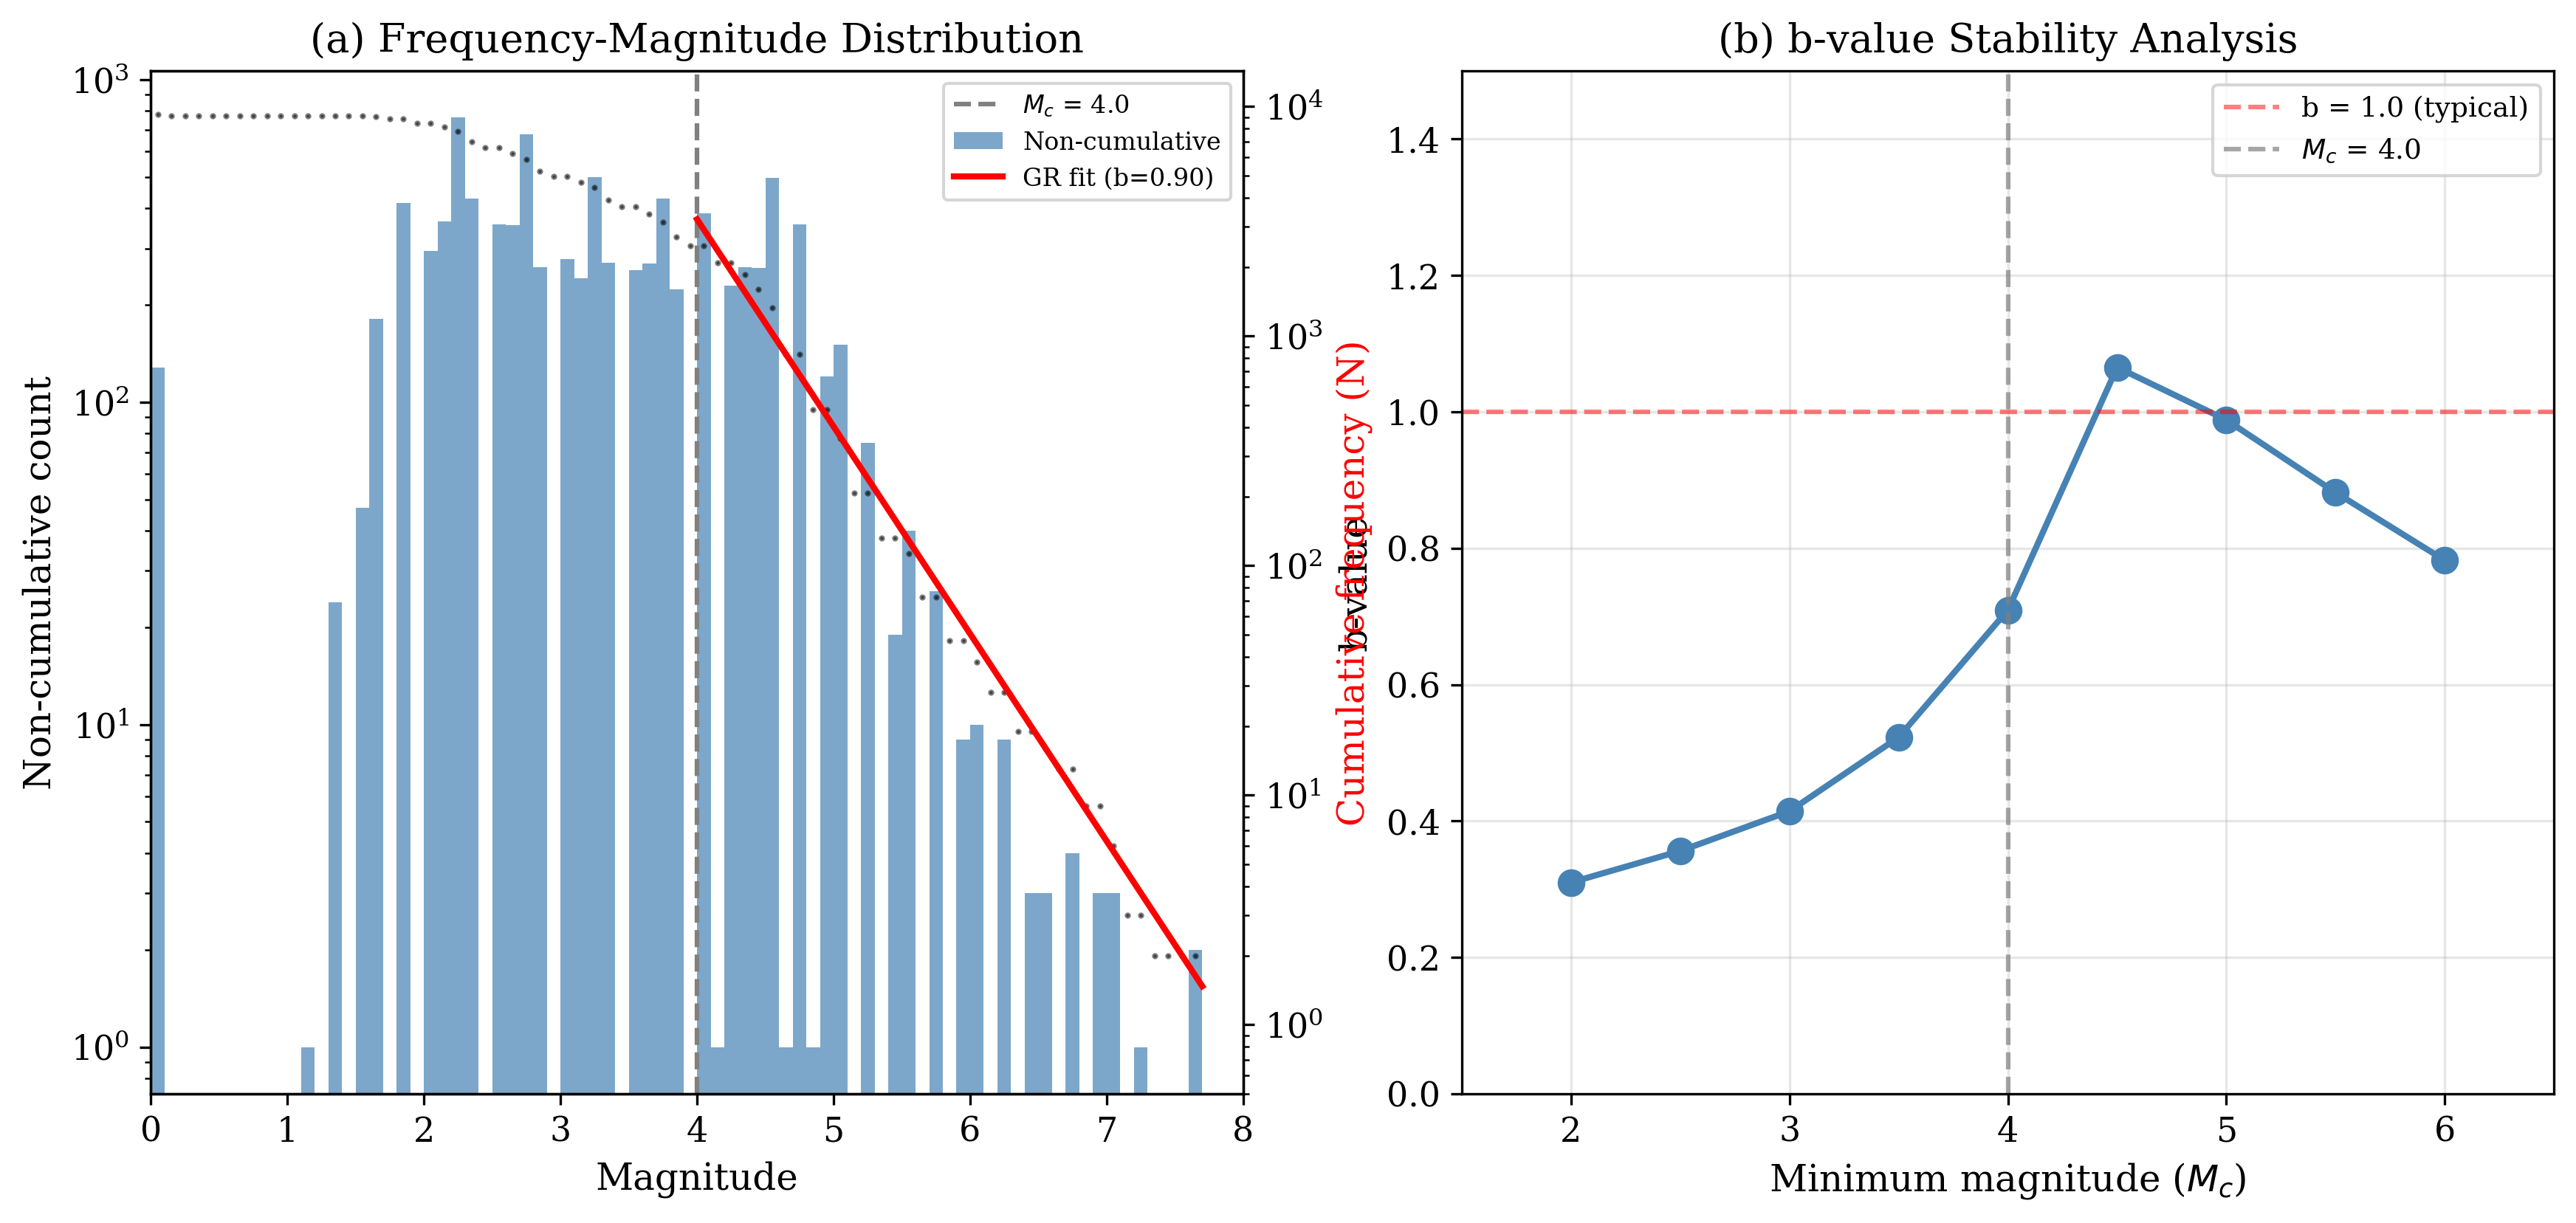
\includegraphics[width=\textwidth]{figures/fig2_fmd.png}
    \caption{(a) Frequency-magnitude distribution for the Myanmar earthquake catalog (1970--2026) with Gutenberg-Richter fit above $M_c$ = 4.0. (b) b-value stability analysis showing convergence to $b \approx 1.0$ at $M_c \geq$ 4.5, confirming catalog incompleteness below M4.}
    \label{fig:fmd}
\end{figure}

The depth distribution (Figure~\ref{fig:depth}) confirms that 74.5\% of events are shallow ($<$30~km), consistent with crustal faulting along the Sagaing Fault.
A secondary population of intermediate and deep events (13.7\%) is associated with the subducting Indian plate beneath western Myanmar.

\begin{figure}[H]
    \centering
    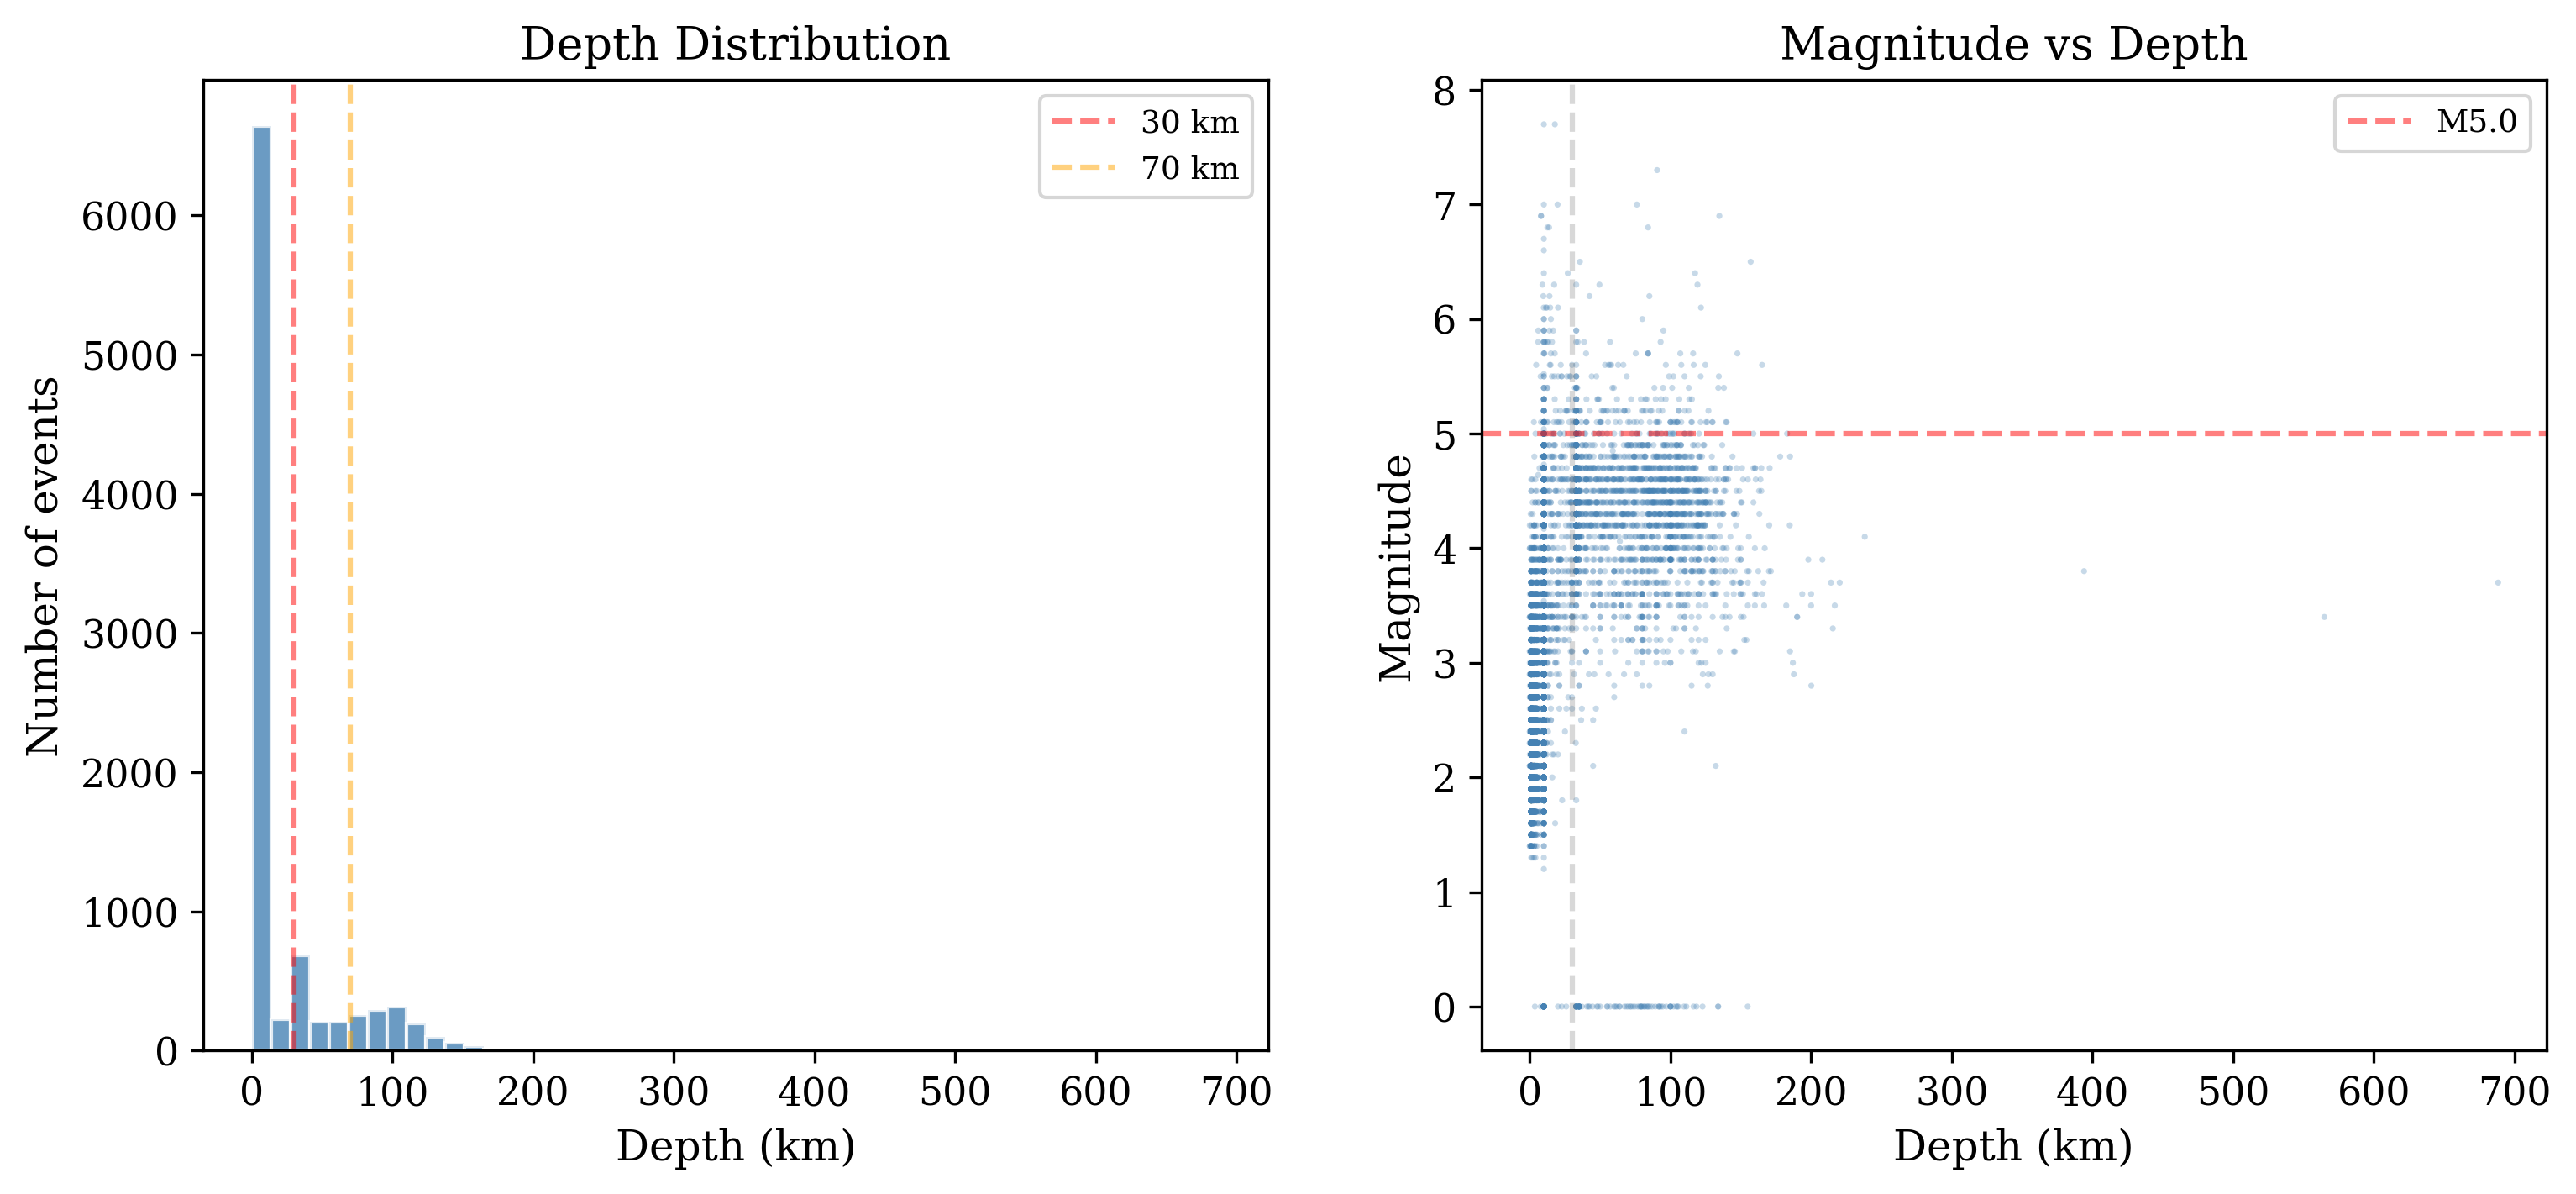
\includegraphics[width=\textwidth]{figures/fig3_depth.png}
    \caption{(a) Depth histogram showing the dominance of shallow seismicity. (b) Magnitude versus depth, indicating that the largest events occur at shallow depths along the crustal fault system.}
    \label{fig:depth}
\end{figure}

Temporal analysis (Figure~\ref{fig:temporal}) shows an increase in detected events over time, primarily reflecting improvements in seismic network coverage rather than changes in seismicity rate.

\begin{figure}[H]
    \centering
    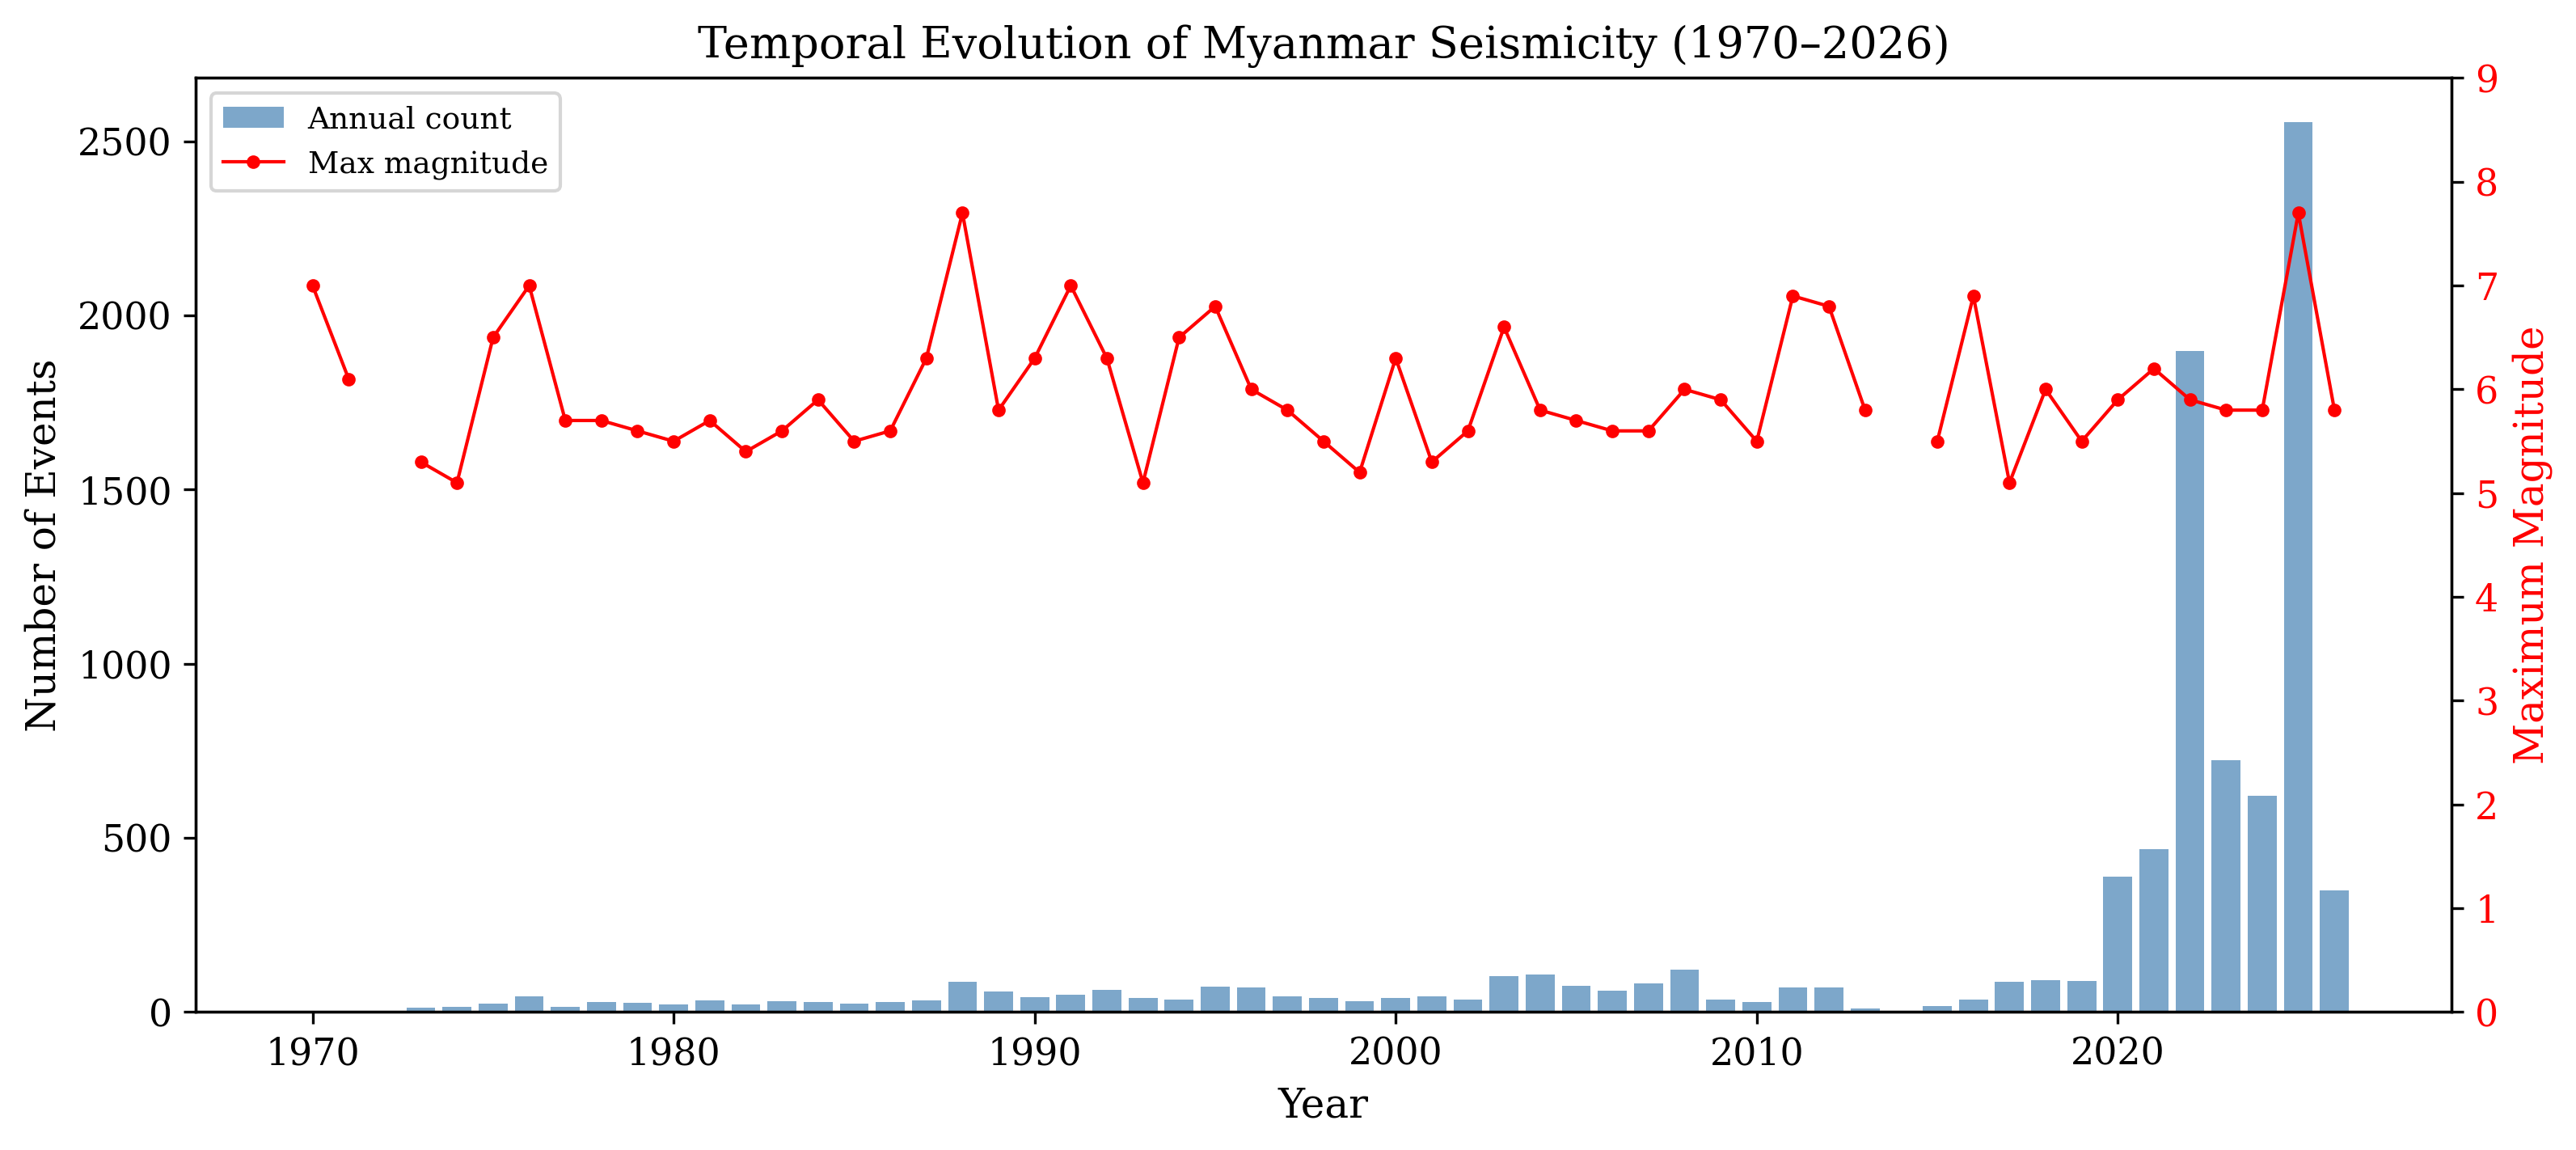
\includegraphics[width=\textwidth]{figures/fig6_temporal.png}
    \caption{Annual earthquake count (bars) and maximum magnitude per year (red line). The increase in small events after 2000 reflects improved network detection capability.}
    \label{fig:temporal}
\end{figure}

\subsection{Spatial Clustering}

UTM-projected DBSCAN identifies seven seismic clusters and 184 noise events (Table~\ref{tab:clusters}).
The dominant Central Myanmar cluster contains 8,775 events (95.0\%) and includes both the 2025 M$_w$ 7.7 Mandalay earthquake and the 1988 M$_w$ 7.7 Lancang--Gengma earthquake, spanning the Mandalay-Sagaing corridor.
The Northern Myanmar (Kachin) cluster contains 109 events with a maximum of M$_w$ 7.0.
The use of projected coordinates ensures that distances are computed correctly in kilometers, avoiding the latitude-dependent distortion inherent in raw degree-based clustering.

\begin{table}[H]
\centering
\caption{DBSCAN clustering results (UTM-projected, $\epsilon = 33.3$~km, min\_samples = 10).}
\label{tab:clusters}
\begin{tabular}{llrrrr}
\toprule
\textbf{Cluster} & \textbf{Region} & \textbf{Events} & \textbf{Max M} & \textbf{Max M Date} & \textbf{Mean Depth (km)} \\
\midrule
0 & Central Myanmar (Mandalay/Sagaing) & 8,775 & 7.7 & 2025-03-28 & 25 \\
1 & N Myanmar (Kachin/Sagaing) & 109 & 7.0 & 1976-05-29 & 29 \\
2 & S Myanmar (Bago/Yangon) & 62 & 5.6 & 1979-10-03 & 36 \\
3 & SE Myanmar (Mon/Kayin) & 69 & 3.9 & 2022-10-18 & 8 \\
4 & NE Myanmar (Shan/Lashio) & 20 & 4.7 & 2023-05-17 & 10 \\
5 & NE Myanmar (Bhamo/Myitkyina) & 12 & 4.8 & 1981-05-14 & 40 \\
6 & E Shan (China Border) & 11 & 4.0 & 2020-09-09 & 9 \\
-- & Unclustered (noise) & 184 & 5.5 & -- & 26 \\
\bottomrule
\end{tabular}
\end{table}

\subsection{PGA Estimation}

PGA values at the 254 dam sites range from 0.022$g$ to 0.201$g$ (mean: 0.062$g$), computed using $R_{jb}$ (distance to fault trace) rather than epicentral distance.
The attenuation curves (Figure~\ref{fig:pga}) show the ASK08 model prediction for M$_w$ 7.7 strike-slip on rock ($V_{S30}$ = 760~m/s).
The model predicts median PGA of 0.14$g$ at $R_{jb}$ = 10~km and 0.05$g$ at $R_{jb}$ = 100~km.

Recorded values from the 2025 event (0.62$g$ at USGS station, 1.07$g$ at GFZ station) exceed the model median by factors of 3--6.
This is expected: the ASK08 model has a within-event standard deviation of $\sigma \approx 0.6$ in natural log units, meaning that recordings at the 84th percentile exceed the median by a factor of $e^{0.6} \approx 1.8$.
The Naypyidaw recordings are at approximately the 95th percentile, consistent with forward directivity effects from the supershear rupture propagation.
The good agreement between the model median and the distribution of dam PGA estimates confirms that the ASK08 model provides a realistic first-order ground motion estimate.

\begin{figure}[H]
    \centering
    
\includegraphics[width=0.75\textwidth]{figures/fig5_pga_attenuation.png}
    \caption{PGA attenuation curves for the Abrahamson \& Silva (2008) GMPE for different magnitudes. Gray dots show PGA at dam sites using $R_{jb}$ to the fault trace. Red diamonds show recorded values from the 2025 event.}
    \label{fig:pga}
\end{figure}

\subsection{Probabilistic Seismic Hazard Curves}

To complement the scenario-based PGA estimates, we compute seismic hazard curves at each dam site using the Cornell-McGuire probabilistic seismic hazard analysis (PSHA) approach.
The Gutenberg-Richter frequency-magnitude relationship (with corrected $b = 0.71$, $a = 6.23$ converted to annual rate) is integrated over magnitude bins from M5.0 to M8.0, with the ASK08 GMPE providing the conditional probability of exceeding each PGA level given each magnitude.
Epistemic uncertainty is captured by the GMPE's within-event standard deviation ($\sigma_{ln} = 0.65$).

Hazard curves for representative dam sites (Figure~\ref{fig:hazard}) show the wide range of seismic exposure across the dam portfolio.
At the closest dam to the fault trace ($R_{jb} = 1$~km), the 475-year PGA (10\% exceedance probability in 50 years) reaches 1.31$g$, while at more distant sites ($R_{jb} \approx$ 9~km) it drops to 0.6--0.9$g$.
Across all 254 dams, the mean 475-year PGA is 0.31$g$, with 32 dams (12.6\%) exceeding 0.5$g$ at the 475-year return period.
These probabilistic estimates are consistent with the scenario-based PGA (mean 0.06$g$ from the M$_w$ 7.7 deterministic event), with the higher probabilistic values reflecting the integration over all possible earthquake magnitudes and the inclusion of ground motion variability.

\begin{figure}[H]
    \centering
    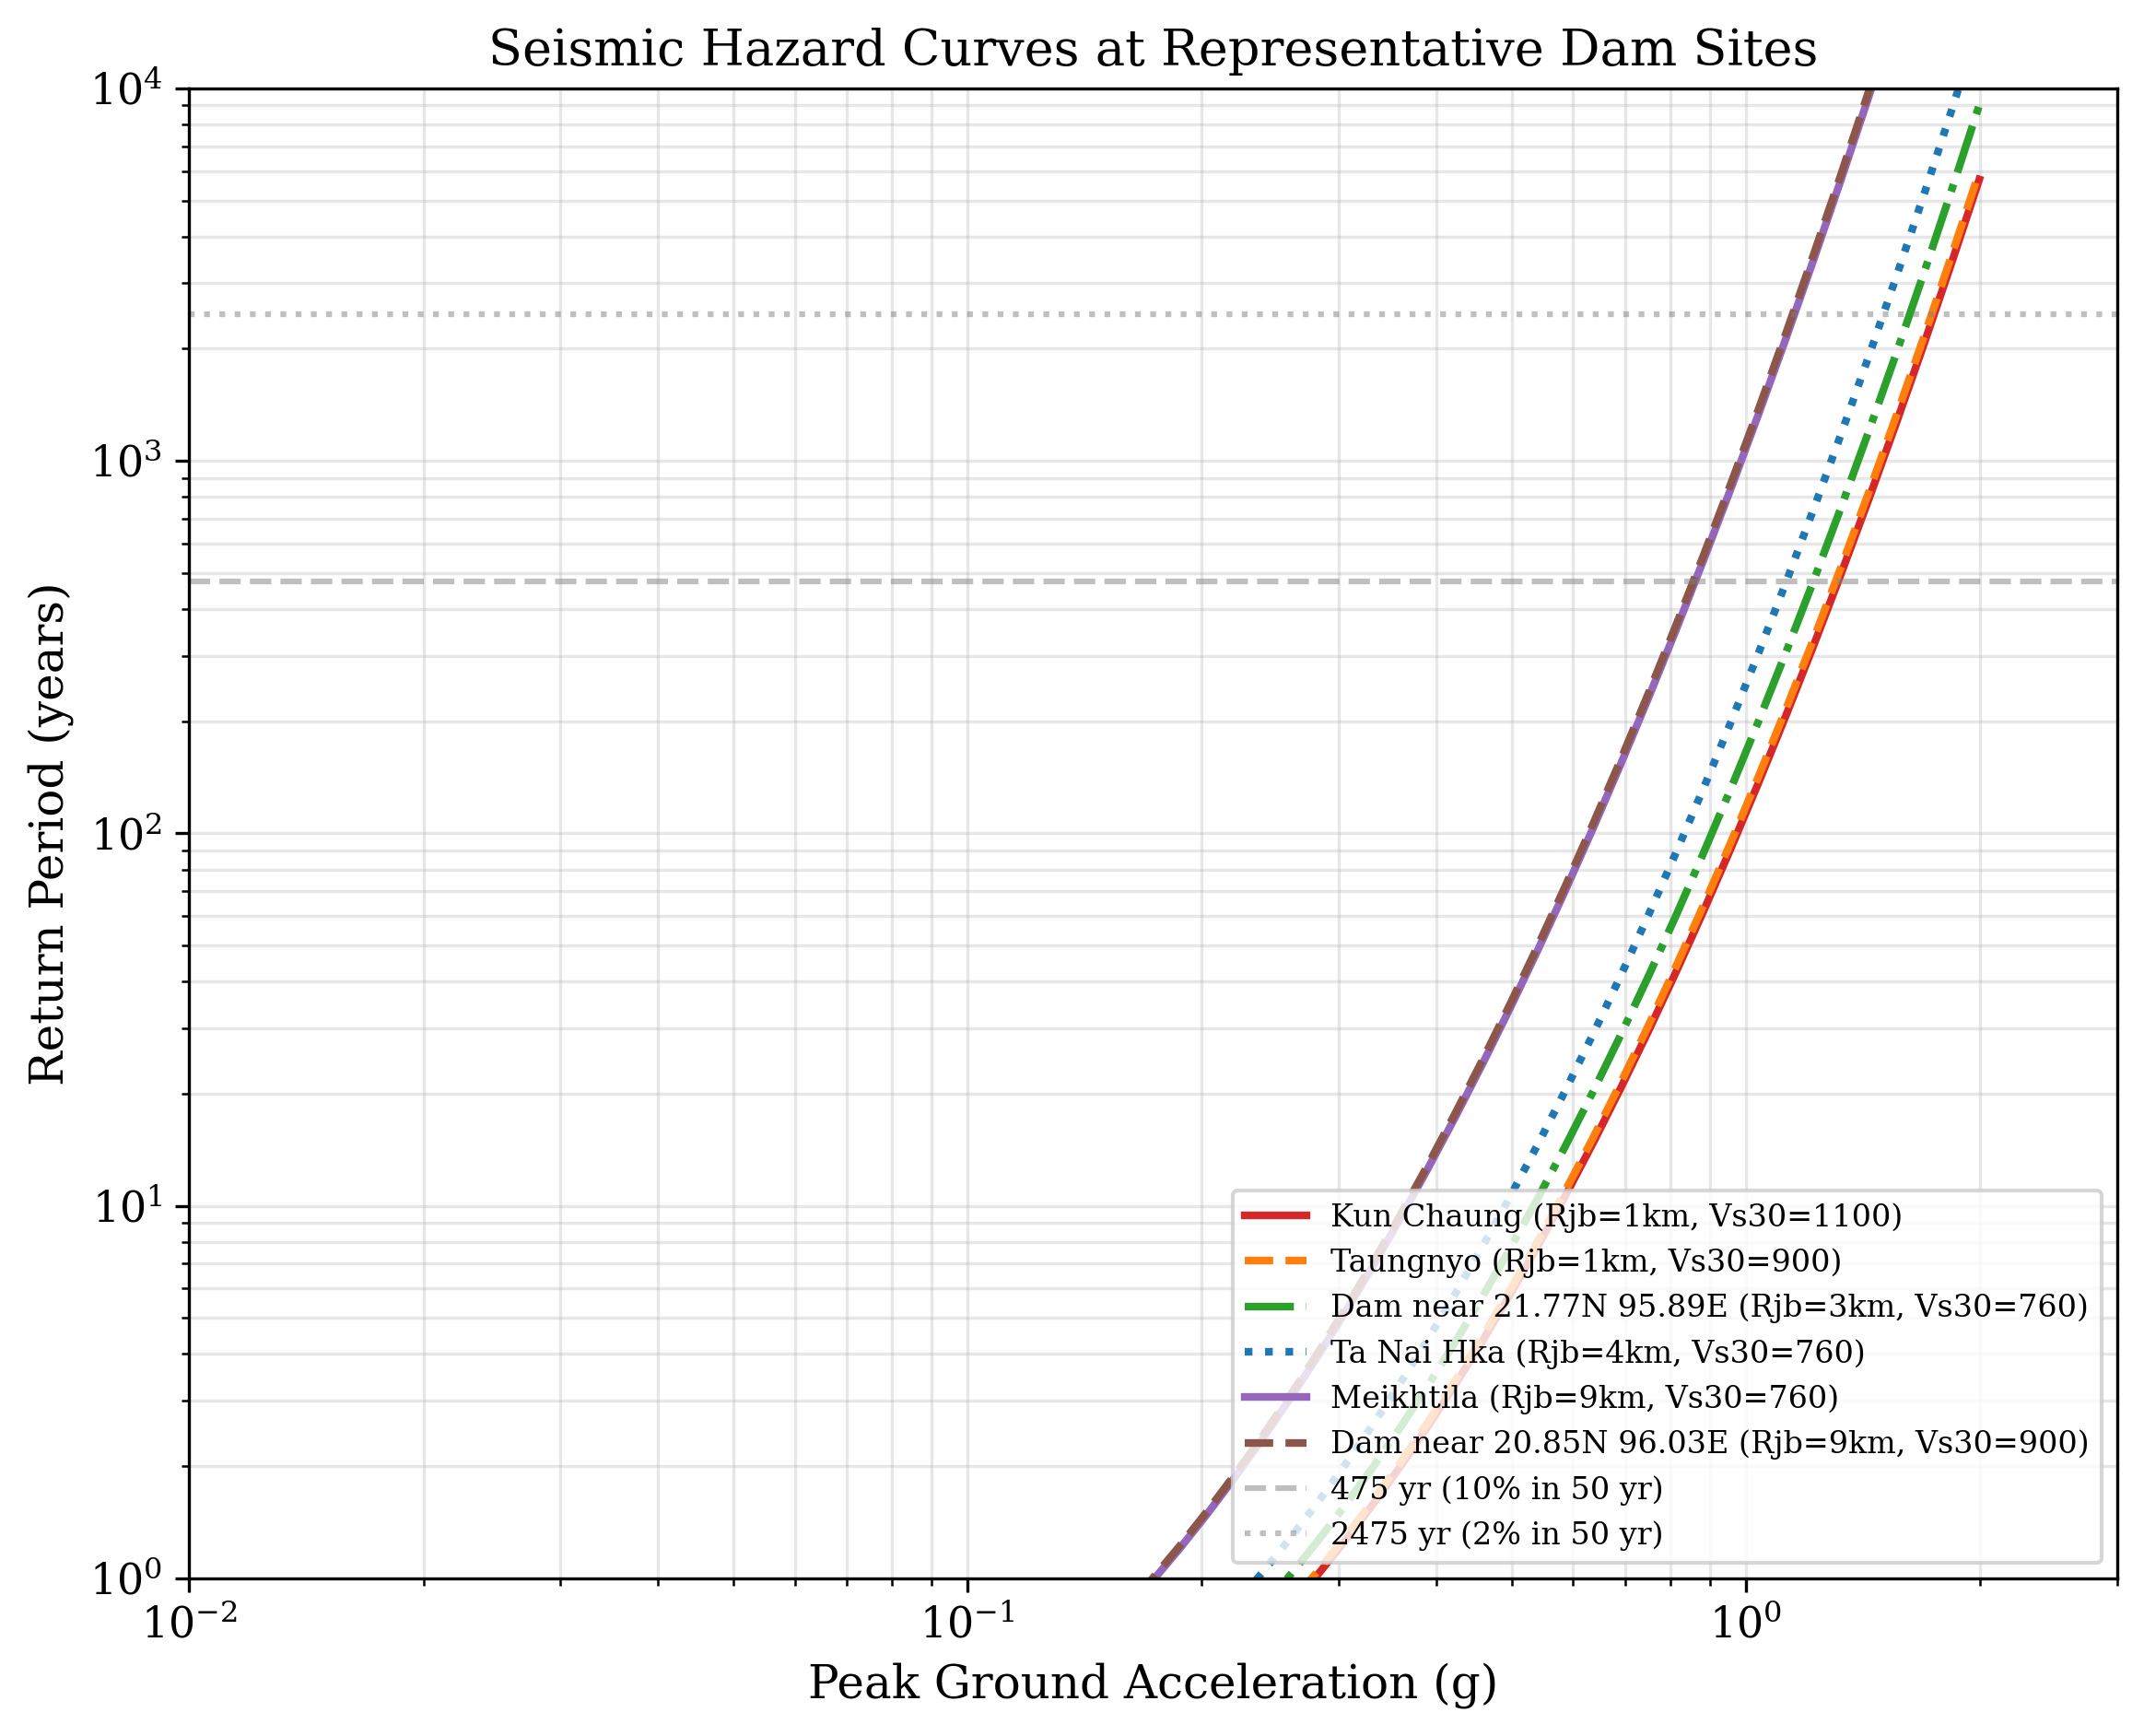
\includegraphics[width=0.85\textwidth]{figures/fig10_hazard_curves.png}
    \caption{Seismic hazard curves (PGA vs return period) at representative dam sites. Dashed lines indicate 475-year (10\% in 50 years) and 2,475-year (2\% in 50 years) return periods.}
    \label{fig:hazard}
\end{figure}

\subsection{Dam Risk Assessment}

The composite risk assessment classifies 25 dams (9.8\%) as \textit{Critical}, 119 (46.9\%) as \textit{High}, 100 (39.4\%) as \textit{Moderate}, and 10 (3.9\%) as \textit{Low} (Figure~\ref{fig:risk_map}, Table~\ref{tab:risk_summary}).
The spatial pattern (Figure~\ref{fig:risk_map}) shows that the highest-risk dams are concentrated along the central Sagaing Fault corridor, where the M$_w$ 7.7 and previous large events have occurred.

\begin{table}[H]
\centering
\caption{Dam risk grade summary.}
\label{tab:risk_summary}
\begin{tabular}{lrrr}
\toprule
\textbf{Risk Grade} & \textbf{Count} & \textbf{Percentage} & \textbf{Score Range} \\
\midrule
Critical & 25 & 9.8\% & $\geq 7.0$ \\
High & 119 & 46.9\% & 5.0--6.9 \\
Moderate & 100 & 39.4\% & 3.0--4.9 \\
Low & 10 & 3.9\% & $< 3.0$ \\
\bottomrule
\end{tabular}
\end{table}

\begin{figure}[H]
    \centering
    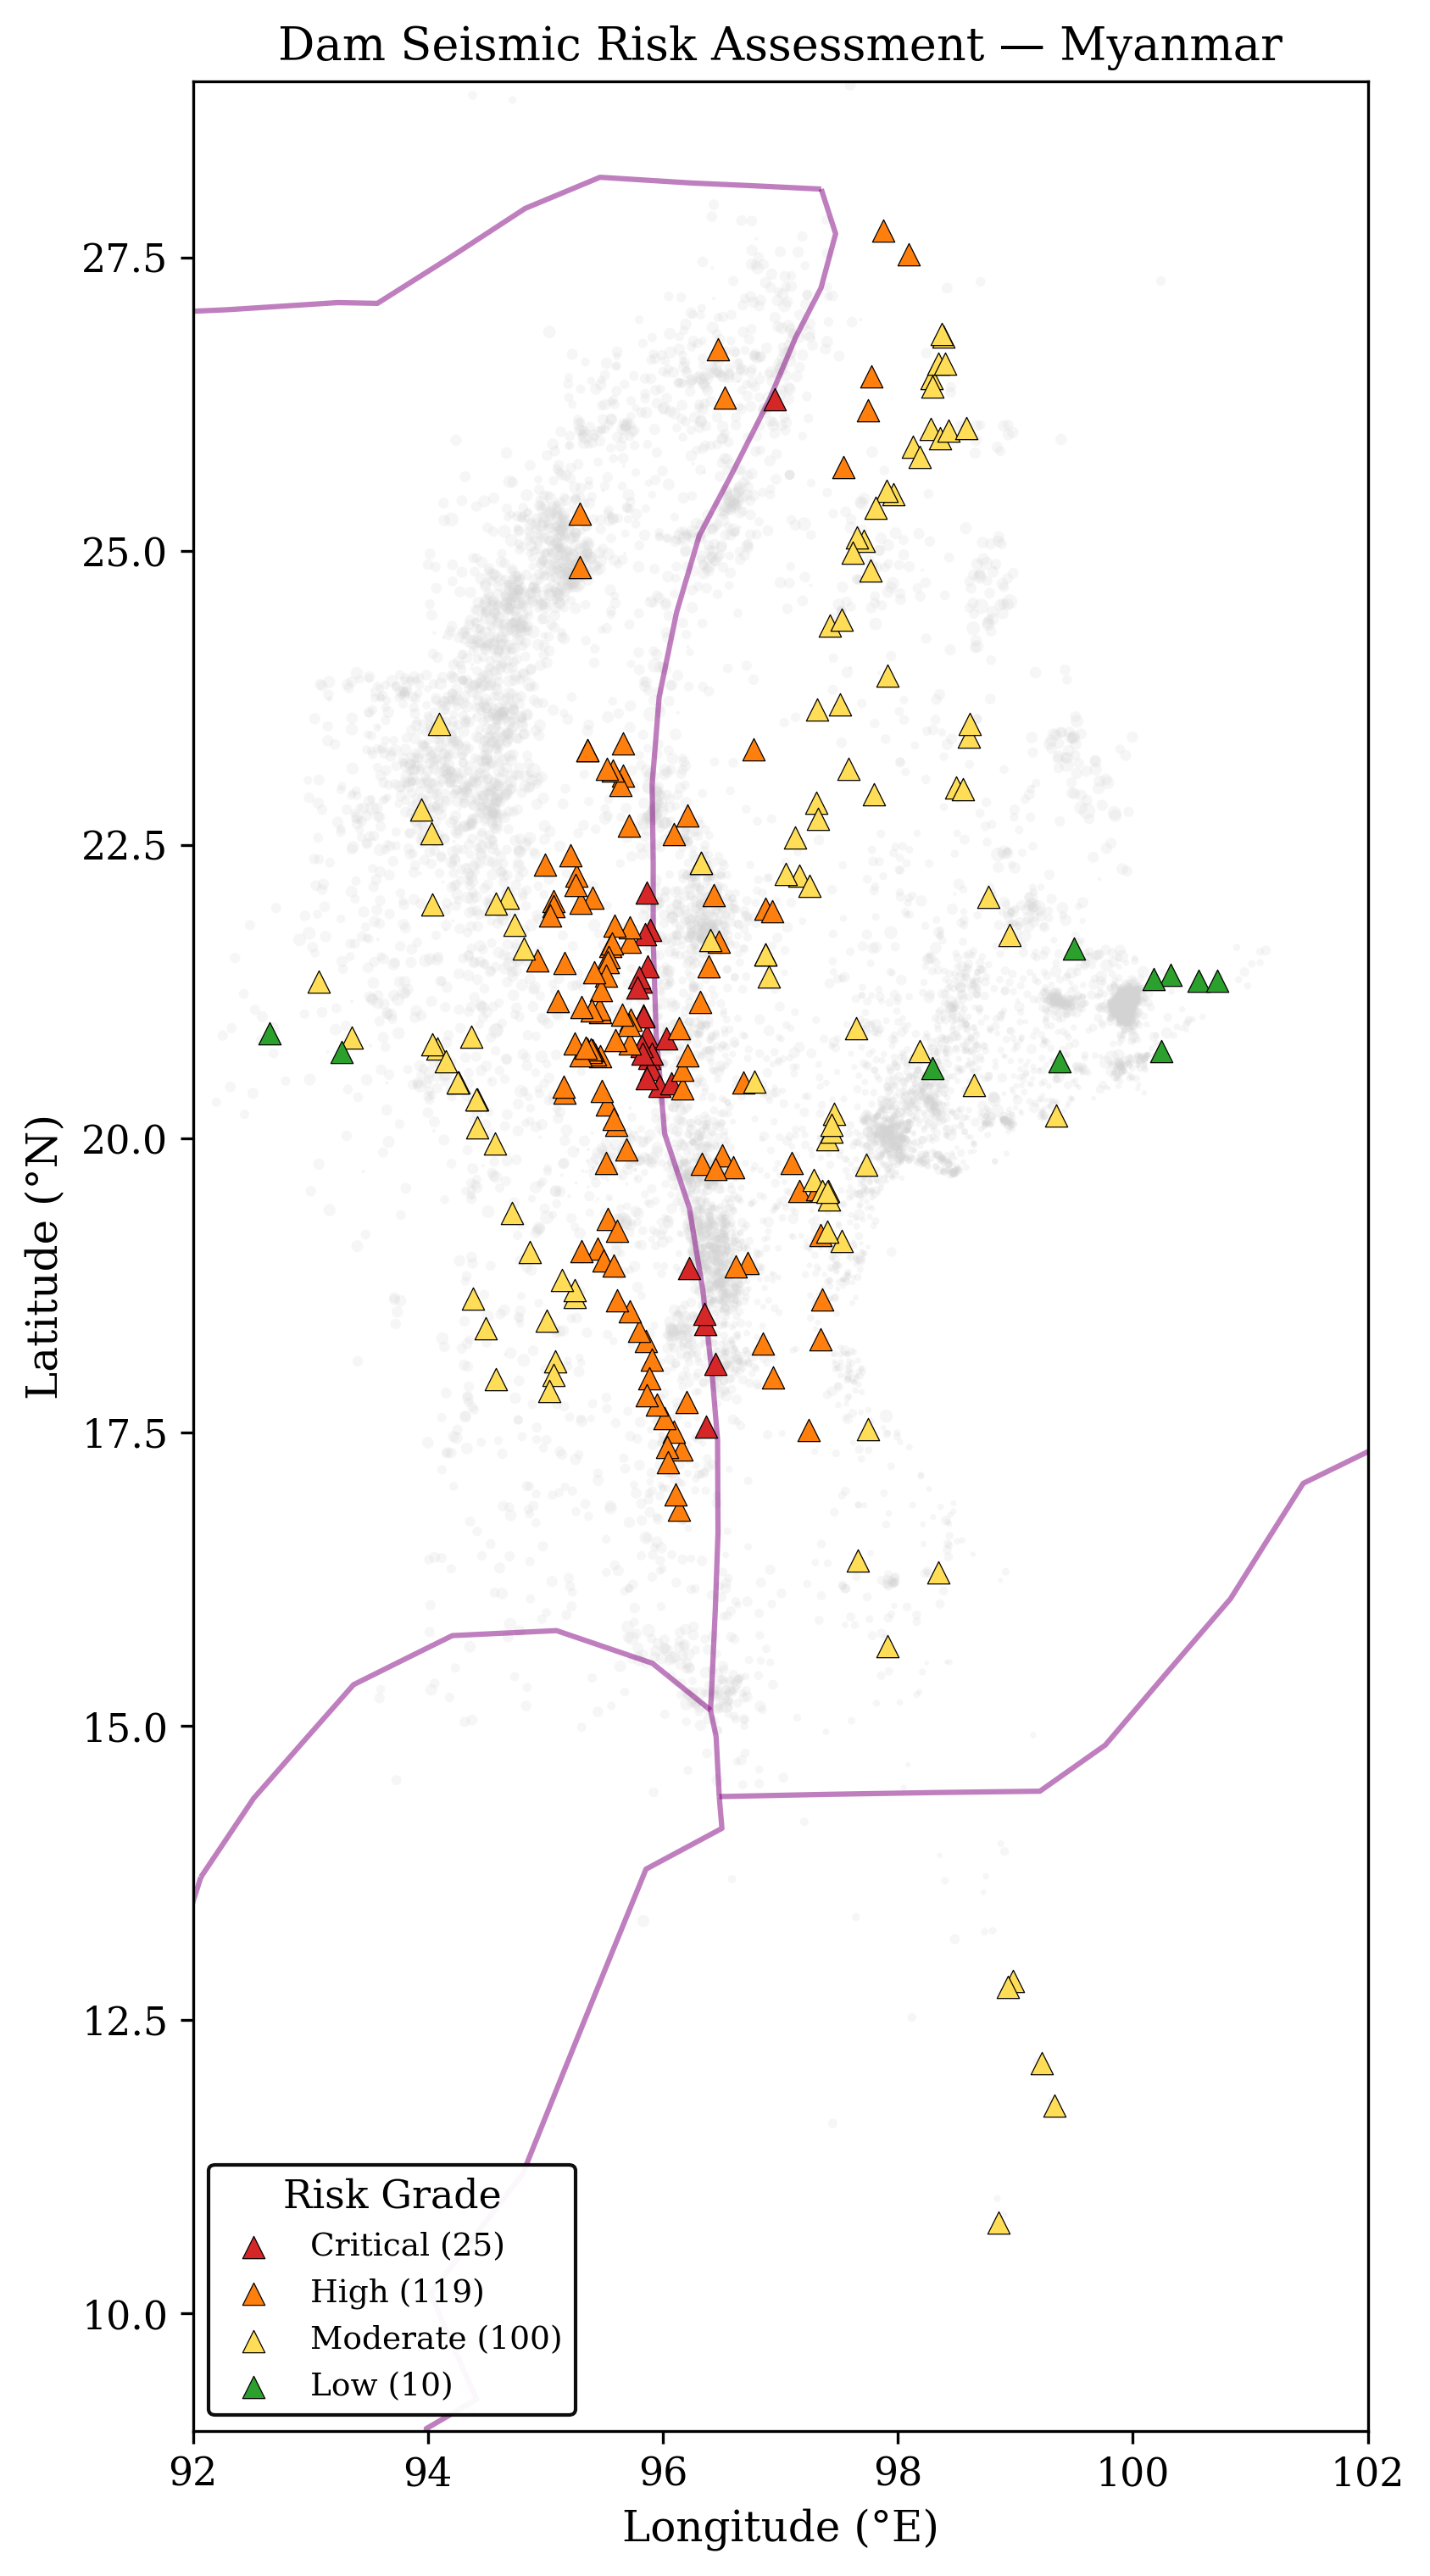
\includegraphics[width=0.9\textwidth]{figures/fig4_dam_risk_map.png}
    \caption{Dam risk assessment map. Triangles show dam locations colored by risk grade. Background shows earthquake distribution. Purple lines indicate fault traces.}
    \label{fig:risk_map}
\end{figure}

\subsection{Sensitivity Analysis}

The Monte Carlo sensitivity analysis (Figure~\ref{fig:risk_dist}c) reveals substantial variability in the grade counts across different weight combinations.
The mean Critical count is 18 $\pm$ 42 (range: 0--208), reflecting the strong dependence of the Critical classification on the seismic and fault proximity weights.
However, the combined Critical+High fraction remains above 30\% across all weight combinations, confirming that a significant majority of Myanmar's dams face elevated seismic risk regardless of the specific weighting scheme.

\begin{figure}[H]
    \centering
    
\includegraphics[width=\textwidth]{figures/fig7_risk_distribution.png}
    \caption{(a) Histogram of composite risk scores for 254 dams. (b) Number of dams in each risk grade category. (c) Monte Carlo sensitivity analysis showing the distribution of grade counts across 100 random weight combinations.}
    \label{fig:risk_dist}
\end{figure}

\subsection{Aftershock Forecast}

The Modified Omori law fit to M$\geq$3.0 aftershocks of the 2025 Mandalay earthquake yields parameters $K = 1.0$, $c = 0.12$~hours, and $p = 0.83$.
The $p$-value is slightly below the typical global average of $\sim$1.0, suggesting a somewhat slower than normal aftershock decay rate.
The cumulative aftershock productivity in our catalog is modest (40 M$\geq$3.0 events within 30 days), though over 500 aftershocks were recorded by regional networks by July 2025 \cite{usgs2025mandalay}.
The discrepancy is attributed to catalog completeness issues in the immediate aftermath of the mainshock and the limited detection capability of the Myanmar seismic network.

\subsection{Population Exposure}

The M$_w$ 7.7 epicentral region exposes approximately 1.77 million people within a 50~km radius, including the cities of Mandalay (1.46M), Sagaing (307K), and Pyin Oo Lwin (166K).
The M$_w$ 6.7 aftershock similarly affects 1.16 million people near Naypyidaw.
Overall, an estimated 38.9 million people (over 70\% of Myanmar's population) were exposed to shaking levels exceeding MMI VI \cite{usgs2025mandalay}.
This highlights the extreme vulnerability of Myanmar's population to seismic events.

\section{Discussion}

\subsection{Catalog Completeness and b-value Interpretation}

The strong dependence of b-value on $M_c$ (Figure~\ref{fig:fmd}b) is the most important methodological finding of this study.
The raw b-value of 0.33 obtained at $M_c$ = 2.2 (the maximum-curvature estimate) is an artifact of catalog incompleteness: the 1970--2000 period has very few events below M4.5, while the post-2020 period records events down to M2.0.
This heterogeneity inflates the apparent proportion of large events.

The corrected b-value of 0.71 at $M_c$ = 4.0 is below the global average of $\approx$1.0 but physically reasonable.
The Sagaing Fault's relatively high rate of M$\geq$7 events (1930, 1931, 1946, 1956, 1991, 2012, 2025) and the 2025 aftershock sequence contribute to the elevated proportion of moderate-to-large events.
We recommend that future studies use only post-2000 or post-2010 data for frequency-magnitude analysis to avoid this incompleteness artifact.

\subsection{Ground Motion Modeling}

The Abrahamson \& Silva (2008) GMPE represents a significant improvement over the previously used Fukushima \& Tanaka (1990) model for three reasons:
(1) it is calibrated for crustal strike-slip earthquakes, matching the Sagaing Fault;
(2) the use of $R_{jb}$ distance properly handles the 500~km extended rupture;
(3) the model median (0.14--0.18$g$ at $R_{jb}$ = 5--10~km) plus one standard deviation ($\times$1.8) encompasses the recorded values (0.62--1.07$g$).

The observed exceedance of the model median by the Naypyidaw recordings is consistent with forward directivity effects from the supershear rupture, which are not explicitly modeled by ASK08.
Future studies should consider directivity-modified GMPEs or the NGA-West2 models (Abrahamson et al. 2014, Boore et al. 2014) which provide improved near-field predictions.

\subsection{Dam Vulnerability}

The finding that 56.7\% of Myanmar's documented dams are classified as Critical or High risk is alarming but not surprising given the country's tectonic setting.
The central Sagaing Fault runs through the heart of Myanmar's agricultural and economic zone, where most dams are located.
This assessment is consistent with the Myanmar government's report that 586 dams were damaged in the 2025 event, far exceeding the 254 dams in our database and suggesting that many additional small dams and weirs exist that are not captured in the Open Development Mekong dataset.

The sensitivity analysis (Figure~\ref{fig:risk_dist}c) shows that while the exact number of dams in each grade varies with weight selection, the overall conclusion --- that a majority of Myanmar's dams face significant seismic hazard --- is robust.

Key concerns include:
\begin{itemize}
    \item Many irrigation dams in the central dry zone are earthen embankments with limited seismic resistance
    \item Hydropower dams in Shan and Kachin States are situated in areas of complex fault geometry
    \item The 2025 event demonstrated that recorded PGA can exceed 1.0$g$ near the fault trace and 0.1$g$ at distances exceeding 100~km
    \item A dam collapse in Mandalay was reported to have caused downstream flooding during the 2025 event
\end{itemize}

\subsection{Limitations}

Several limitations should be acknowledged:
\begin{enumerate}
    \item The earthquake catalog is heterogeneous, with detection thresholds varying over time and space; while we correct for this by using $M_c$ = 4.0, residual incompleteness may affect the b-value
    \item Site effects (soil amplification, topographic effects, basin resonance) are not considered; all PGA estimates assume NEHRP BC rock ($V_{S30}$ = 760~m/s)
    \item Dam structural properties (age, construction quality, foundation conditions) are not available in the dataset
    \item The risk scoring uses simplified weighting that is tested via sensitivity analysis but not validated against actual damage data
    \item The dam database (254 structures) is incomplete; the government reported 586 damaged dams, suggesting the true number is at least double our dataset
    \item Our aftershock catalog captures only a fraction of the 500+ events recorded by regional networks
    \item The ASK08 model does not account for directivity effects, which may cause systematic underestimation in the forward directivity direction of the supershear rupture
\end{enumerate}

Despite these limitations, the results provide a valuable first-order screening of dam vulnerability in Myanmar and identify priority structures for detailed site-specific evaluation.

\subsection{Recommendations}

Based on our findings, we recommend:
\begin{enumerate}
    \item Immediate structural inspection of the 25 Critical-risk dams, prioritizing those closest to the Sagaing Fault
    \item Comprehensive dam inventory to capture the hundreds of small dams and weirs not included in existing databases
    \item Installation of strong-motion accelerographs at all dams within 100~km of the fault trace
    \item Development of site-specific probabilistic seismic hazard assessments (PSHA) using NGA-West2 GMPEs calibrated for Myanmar
    \item Emergency action plans for downstream communities, particularly for dams above major population centers
    \item Incorporation of dam safety considerations into Myanmar's national building code
    \item Use of the 2025 recorded ground motions (PGA up to 1.07$g$) to validate and calibrate future attenuation models for the region
\end{enumerate}

\section{Conclusions}

We present a comprehensive seismic risk assessment of Myanmar's dam infrastructure following the devastating 2025 M$_w$ 7.7 Mandalay earthquake.
Key methodological improvements over previous work include: (1) corrected b-value estimation with catalog completeness analysis; (2) modern GMPE (ASK08) appropriate for crustal strike-slip with site-specific $V_{S30}$ from Copernicus DEM; (3) UTM-projected DBSCAN clustering; (4) Monte Carlo sensitivity analysis; (5) probabilistic seismic hazard curves at each dam site.
Our analysis of 9,242 earthquakes and 254 dams yields the following key findings:
\begin{enumerate}
    \item The corrected Gutenberg-Richter b-value is 0.71 at $M_c$ = 4.0; the previously reported b = 0.33 was an artifact of catalog incompleteness
    \item b-value stability analysis confirms that the catalog is only complete above $M_c \approx$ 4.0--4.5 for the full 1970--2026 period
    \item Seven distinct seismic zones are identified using UTM-projected DBSCAN, with the Central Myanmar cluster accounting for 95\% of events
    \item 56.7\% of Myanmar's documented dams (144 out of 254) are classified as Critical or High seismic risk
    \item PGA at dam sites ranges from 0.022$g$ to 0.201$g$ using the ASK08 model with $R_{jb}$ to the fault trace, consistent with recorded ground motions when within-event variability is considered
    \item Monte Carlo sensitivity analysis confirms that the finding of widespread dam vulnerability is robust to weight perturbation
    \item The 2025 earthquake's 500~km supershear rupture demonstrates that a single event can threaten dam infrastructure across the entire central Myanmar corridor
    \item An estimated 1.77 million people are exposed within 50~km of the M$_w$ 7.7 epicenter, and 38.9 million were exposed to shaking exceeding MMI VI
\end{enumerate}

These results underscore the urgent need for seismic safety evaluation of Myanmar's dam infrastructure, particularly in the aftermath of the 2025 earthquake.
All data, analysis code, and interactive visualizations are available as open-source tools at \url{https://github.com/akzedevops/mmeqopendata}.

\section*{Data Availability}

All earthquake data is available through the Myanmar Earthquake API (\url{https://mmeq.akze.net}).
Dam data is available from Open Development Mekong (\url{https://data.opendevelopmentmekong.net/en/dataset/myanmar-dams}), licensed CC BY-SA 4.0.
The analysis toolkit is open-source under the MIT License.

\section*{Acknowledgments}

Earthquake data is aggregated from USGS, GFZ, ISC, and regional seismic networks.
Dam data is sourced from the International Finance Corporation (IFC) and CGIAR's Water, Land, and Ecosystems (WLE) program through Open Development Mekong.
The author acknowledges the USGS, Thai Meteorological Department, and GFZ for their rapid release of data following the 2025 Mandalay earthquake.

\bibliographystyle{unsrt}
\begin{thebibliography}{20}

\bibitem[abrahamson2008]{abrahamson2008}
Abrahamson, N. A. and Silva, W. J. (2008).
Summary of the Abrahamson \& Silva NGA ground-motion relations.
\textit{Earthquake Spectra}, 24(1):67--97.

\bibitem[ester1996]{ester1996density}
Ester, M., Kriegel, H.-P., Sander, J., and Xu, X. (1996).
A density-based algorithm for discovering clusters in large spatial databases with noise.
In \textit{Proceedings of the 2nd International Conference on Knowledge Discovery and Data Mining}, pages 226--231.

\bibitem[gutenberg1944]{gutenberg1944frequency}
Gutenberg, B. and Richter, C. F. (1944).
Frequency of earthquakes in California.
\textit{Bulletin of the Seismological Society of America}, 34(4):185--188.

\bibitem[hurukawa2011]{hurukawa2011two}
Hurukawa, N. and Maung, P. M. (2011).
Two seismic gaps on the Sagaing Fault, Myanmar, derived from relocation of historical earthquakes since 1918.
\textit{Geophysical Research Letters}, 38(L01310).

\bibitem[odmekong2018]{odmekong2018}
Open Development Mekong (2018).
Myanmar Dams dataset.
\url{https://data.opendevelopmentmekong.net/en/dataset/myanmar-dams}. CC BY-SA 4.0.

\bibitem[robinson2010]{robinson2010earthquake}
Robinson, D. P., Das, S., and Searle, M. P. (2010).
Earthquake fault superhighways.
\textit{Tectonophysics}, 493(3--4):236--243.

\bibitem[socquet2006]{socquet2006myanmar}
Socquet, A., Vigny, C., Chamot-Rooke, N., Simons, W., Rangin, C., and Ambrosius, B. (2006).
India and Sunda plates motion and deformation along their boundary in Myanmar determined by GPS.
\textit{Journal of Geophysical Research: Solid Earth}, 111(B5).

\bibitem[utsu1961]{utsu1961statistical}
Utsu, T. (1961).
A statistical study on the occurrence of aftershocks.
\textit{Geophysical Magazine}, 30:521--605.

\bibitem[usgs2025]{usgs2025mandalay}
USGS (2025).
M 7.7 -- 14 km NNW of Sagaing, Myanmar.
\url{https://earthquake.usgs.gov/earthquakes/eventpage/us7003sbx2}.

\bibitem[vigny2003]{vigny2003present}
Vigny, C., Socquet, A., Rangin, C., Chamot-Rooke, N., Pubellier, M., Bouin, M.-N., Bertrand, G., and Becker, M. (2003).
Present-day crustal deformation around Sagaing fault, Myanmar.
\textit{Journal of Geophysical Research: Solid Earth}, 108(B11).

\bibitem[wald2007]{wald2007}
Wald, D. J. and Allen, T. I. (2007).
Topographic slope as a proxy for seismic site conditions and amplification.
\textit{Bulletin of the Seismological Society of America}, 97(5):1379--1395.

\bibitem[wang2014]{wang2014active}
Wang, Y., Sieh, K., Aung, T., Min, S., Khaing, S. N., and Tun, S. T. (2014).
Active tectonics and earthquake potential of the Myanmar region.
\textit{Journal of Geophysical Research: Solid Earth}, 119(4):3767--3822.

\bibitem[wiemer2000]{wiemer2000minimum}
Wiemer, S. and Wyss, M. (2000).
Minimum magnitude of completeness in earthquake catalogs: Examples from Alaska, the western United States, and Japan.
\textit{Bulletin of the Seismological Society of America}, 90(4):859--869.

\end{thebibliography}

\end{document}
